\documentclass[letterpaper,10pt]{article}
\usepackage[bookmarks]{hyperref}
\usepackage[utf8]{inputenc}
\usepackage[english]{babel}

% sans serif
\renewcommand*{\familydefault}{\sfdefault}

% pictures!
\usepackage{graphicx}
    % \begin{figure}[p]
    %     \centering
    %     \includegraphics[width=0.8\textwidth]{image.png}
    %     \caption{Awesome Image}
    %     \label{fig:awesome_image}
    % \end{figure}

% math++
\usepackage{mathtools}

\usepackage{tabularx}

% bold all column
\usepackage{array}

\usepackage{amsfonts}

% compact lists (compactitem, compactenum, compactdesc)
\usepackage{paralist}

% nicer tables
\usepackage{booktabs}

% layout
\usepackage{float}

% sans serif math
\usepackage{arevtext,arevmath}

% chemical equations
\usepackage{mhchem}
\usepackage{chemfig}

% text columns
\usepackage{multicol}

% dummy text
\usepackage{lipsum}

% frames around text
\usepackage{mdframed}

% section style
\usepackage{sectsty}

% margins
\usepackage[top=0.25in, bottom=0.25in, left=0.25in, right=0.25in]{geometry}

% per-section toc
\usepackage[insection]{minitoc}

% compact list, reduce margins
% \setlist[compactdesc]{itemindent=10pt}

\mdfsetup{nobreak=false} %, rightline=false, leftline=false}

% style
\restylefloat{table}
\sectionfont{\rmfamily}
\subsectionfont{\rmfamily\centering}

%ceiling/floor. use \ceil*{stuff} to scale symbols
\DeclarePairedDelimiter\ceil{\lceil}{\rceil}
\DeclarePairedDelimiter\floor{\lfloor}{\rfloor}

\graphicspath{{pngs/}}

\begin{document}

\title{Chemistry 121/122 notes}
\author{Hugo Rivera}
\date{2014 - 2015}
\maketitle

\dosecttoc
\setlength{\mtcindent}{5pt}
\begin{multicols}{2}
\tableofcontents
\end{multicols}

\section{Chapter 1. Units and Significant Figures}

{\footnotesize
\begin{multicols}{3}
\begin{compactenum}
    \item Elements,  compounds,  hetero/homogeneous mixtures
    \item Common elements
    \item Common prefixes
    \item Significant figures OHYEA
    \item SI units and non-SI units common in chemistry
\end{compactenum}
\end{multicols}
}

\begin{mdframed}
\begin{multicols}{2}
\begin{compactdesc}
    \item[Common elements] C, F, H, N, I, O, P, S, Al, Br, Ca, Cl, He, Li, Mg, Si, Cu, Fe, Pb,
        Hg, K, Ag, Na, Sn
    \item[Common prefixes] Yocto (15),  Tera,  Giga,  Mega,  kilo,  deci,  centi,
        mill,  $\mu$icro,  nano,  \r{A}ngstrom(-10,  non-SI),  p,  femto (-15),  atto,
        zepto (-21)
    \item[SI units] kg, m, s or sec, K, mol, A, cd (candela)
    \item[Common in chem:] L, 1000 cubic centimeters
    \item[Sig.fig. addition] keep lowest decimal sig.fig.s. $1.0 + 221.31 = 222.3$
    \item[Sig.fig. multiplication] keep lowest sig.fig.s
    \item[Sig.fig. logarithms] sig.figs of mantissa expressed in scientific
        notation equals the number of significant figures to the right of the decimal
        $\log(2.73 ×10^5) = \log(2.73) + \log(10^5) = 0.436 - 5.00000...$.
\end{compactdesc}
\end{multicols}
\end{mdframed}

\section{Chapter 2. Atoms, Molecules, Ions}

\secttoc

{\footnotesize
\begin{multicols}{3}
\begin{compactenum}
    \item Dalton's atomic theory
    \item Key experiments that led to discovery of atom/nucleus/electrons
        (Cathode ray, oil drop, $\alpha$ scattering)
    \item Electrical charge and relative masses of $e^-, p^+, n$
    \item Subatomic composition of isotopes
    \item Atomic weight knowing natural abundances
    \item Periodic table properties, metals/nonmetals
    \item Molecular and ionic substances, in terms of their composition
    \item Empirical/molecular formulas
    \item Compositions expressed as molecular and structural formulas
    \item Ions and the gain/loss of $e^-$, predict common charges
    \item Write empirical formulas of ionic compounds given charges of component ions
    \item Name ionic compounds
    \item Name binary inorganic compounds and acids
    \item Name alkanes and alcohols
\end{compactenum}
\end{multicols}
}
\begin{mdframed}
\begin{multicols}{3}
\subsection{Basics}
\begin{compactdesc}
\item[Empirical formula] extra information is needed to find chemical formula
\item[Mass of electron] $9.10 \cdot 10^{-28}g$
\item[Charge of electron] $1.602 \cdot 10^{-19}C$
\item[Rays] $\beta$ are negative, $\alpha$ are positive, and $\gamma$ are
    neutral.
\item[Cations] positive. meow
\item[Anions] negative.
\end{compactdesc}
\end{multicols}
\end{mdframed}







\begin{mdframed}
\subsection{Dalton's Theory and its Development}
\begin{multicols}{2}
\begin{compactdesc}
\item[Laws:] elements made of atoms, atoms are unique/exclusive to elements,
    atoms cannot be changed by chemistry, compounds have the same relative
    number and kinds of atoms, and the next law:
\item[Law of multiple proportions] elements $A$ and $B$ form two compounds $C_1$
    and $C_2$. This proportion will be a natural number: $\frac{C_1.A}{C_2.A}$
    where $C_1$ is larger.
\item[Cathode rays] cathode rays are electrically charged and negative.
    Determined by firing such a ray and manipulating its positive end using
    magnetic and electric fields
\item[Oil drop experiment] Rate of oil drops affects their rate of descent.
    Used to find ratio of electron's mass and charge.
\item[Rutherford's $\alpha$ scattering] most $\alpha$ particles went through
    a gold foil with little deflection, though some were greatly repelled.
\end{compactdesc}
\end{multicols}
\end{mdframed}



\begin{mdframed}
\subsection{Naming}
\begin{multicols}{2}
Chromate is \ce{CrO4^{2-}}
and Dichromate is \ce{Cr2O7^{2-}}. Permanganate is \ce{MnO4^-}.
Also, the only nonmetal cation encountered is Ammonium \ce{NH4+}.

    \subsubsection{Cations}
    \begin{compactdesc}
    \item[Metal single charge] name ion
    \item[Metal ambiguous charge] name (charge in Roman numerals) ion
    \end{compactdesc}

    \subsubsection{Anions}
    \begin{compactdesc}
    \item[Single] name-ide
    \item[Oxyanions normal sequence] \ce{CO3^{2-}}, \ce{NO3^-}, \ce{ClO3^-};
        \ce{PO4^{3-}}, \ce{SO4^{2-}}
    \item[Oxyanions +1 O count] per-name-ate
    \item[Oxyanions normal O count] name-ate
    \item[Oxyanions -1 O count] name-ite
    \item[Oxyanions -2 O count] hypo-name-ite
    \item[Oxyanions with hydrogen] prepend ``hydrogen'' or ``dihydrogen'' to
        oxyanion name
    \end{compactdesc}

    \subsubsection{Binary compound}
    \begin{compactdesc}
    \item[Greek prefix] to indicate atomic number, leave first alone if AN = 1
    \item[Leftmost first] unless oxygen and a halogen, except \ce{F}.
    \item[Bottommost first]
    \item[Suffix -ide] on second element
    \end{compactdesc}

    \subsubsection{Acids} make \ce{H^+} in water.
    \begin{compactdesc}
    \item[name-ide is converted to] hydro-name-ic acid
    \item[name-ate] is converted to name-ic acid
    \item[name-ite] is converted to name-ous acid
    \end{compactdesc}
\end{multicols}
\end{mdframed}





\begin{mdframed}
\subsection{Alkanes and Alcohols}
\begin{multicols}{2}
\begin{compactdesc}
\item[General formula] \ce{C_nH_{2n + 2}}
\item[Naming sequence] methanol, ethanol, propanol, tetranol, pentanol,
    greek-prefix-nol.
\item[Alcohols] one of the \ce{H} in the alkane replaced by a hydroxide
    \ce{OH}.
\item[Enantiomers] different structure (even if rotated) due to location of the
    hydroxide group. 1-propanol has \ce{OH} on edge, 2-propanol has it in
    center
\end{compactdesc}
\end{multicols}
\end{mdframed}







\section{Chapter 3. Chemical Reactions and Reaction Stoichiometry}

\secttoc

{\footnotesize
\begin{multicols}{3}
\begin{compactenum}
    \item Balance chemical equations
    \item Combination, cdecomposition, combustion reactions
    \item Formula weights
    \item Grams and moles
    \item Avogadro's number
    \item Empirical and molecular formulas of a compound from percentage composition and MW
    \item ID limiting reactants and calculate amounts consumed/formed
    \item Percent yield of a reaction
\end{compactenum}
\end{multicols}
}

\begin{mdframed}
\begin{multicols}{2}
\subsection{Chemical Equations and Reactions}
\begin{compactdesc}
\item[Unbalanced Formula] \ce{CH4 + O2 -> CO2 + H2O}
\item[Balanced Formula] \ce{CH4 + 2O2 -> CO2 + 2H2O}
\item[State indicators] (s), (l), (g), (aq) indicates dissolution in water,
    others for different solvents
\item[Formula weight]
    $\sum_\text{Element} \#\text{E} \cdot \text{E atomic weight}$
\item[Elemental Composition] $\frac{\text{\# element} \cdot \text{weight of}}
                                   {\text{formula weight}}$
\item[] empirical formula weight divided by the molecular weight is always
    a natural number
\item[Combination reaction] \ce{A + B -> C}
\item[Decomposition reaction] \ce{C -> A + B}
\item[Limiting Reactants] test each reaction by moles until an obvious limit is
    found
\item[One AMU] is one $\frac{g}{mol}$.
\end{compactdesc}
\end{multicols}
\end{mdframed}






\begin{mdframed}
\begin{multicols}{2}
\subsection{Stoichiometry}
\begin{compactdesc}
\item[One mole] is equal to $6.022 \cdot 10^{23}$ units.
\item[Stoichiometric Equivalence] \ce{A + 2B -> 3C + 4D} one mole of A
    yields 3 moles of C, one mole of D must have consumed half a mole of B.
\item[Combustion analysis] \ce{\dots C \dots H -> nCO2 + mH2O}
    \%C = $\frac{\text{C}mol}{X mol}$
    \%H = $\frac{\text{H}mol}{X mol}$.
    Try different denominators X until all are natural numbers.
    Use algebra if another element involved.
\item[Percentage yield] actual yield divided by theoretical yield.
\end{compactdesc}
\end{multicols}
\end{mdframed}





\section{Chapter 4. Reactions in Aqueous Solution}

\secttoc

{\footnotesize
\begin{multicols}{3}
\begin{compactenum}
    \item ID compounds as acids or bases, strong weak or non-electrolyte?
    \item Recognize reaction types, simple acid-base, precipitation and
        redox (OILRIG) reactions
    \item Calculate molarity, use it to find volume and moles
    \item Carry out a dilution to achieve a desired solution
    \item Perform and interpret results of a titration
\end{compactenum}
\end{multicols}
}


\begin{mdframed}
\subsection{Solubility Guidelines}
\begin{multicols}{2}
\begin{tabular}{ll}
    soluble & exceptions                                    \\
    \hline
    \ce{NO3^-}                                     &        \\
    \ce{CH3COO^-}                                  &        \\
    alkali metals                                  &        \\
    \hline
    all following & unless with \ce{Hg2^{2+}}, \ce{Pb^{2+}} \\
    \ce{Cl^-}      & unless with \ce{Ag+}                   \\
    \ce{Br^-}      & unless with \ce{Ag+}                   \\
    \ce{I^-}       & unless with \ce{Ag+}                   \\
    \ce{SO4^{2-}}  & unless with \ce{Sr^{2+}}, \ce{Ba^{2+}} \\
\end{tabular}

\begin{tabular}{ll}
 insoluble  & exceptions \\
\hline
 all  following & unless with \ce{NH4+}, alkali metal \\
 \ce{CO3^{2-}}  &  \\
 \ce{PO4^{3-}}  &  \\

 all following & unless with \ce{Ca^{2+}}, \ce{Sr^{2+}}, \ce{Ba^{2+}}  \\
 \ce{S^{2-}} &  \\
 \ce{OH^-}   &  \\
\end{tabular}
\end{multicols}


\subsection{Strong Acids and Bases}
\begin{compactdesc}
\item[Strong acids] HI, HBr, HCl, \ce{HClO3}, \ce{HClO4}, \ce{HNO3}, \ce{H2SO4} (first proton only)
\item[Strong bases] group 1A metal hydroxides \ce{KOH}, group 2A heavy metal
    hydroxides (beginning at \ce{Ca(OH)2})
\item[Weak acids, bases] all else
\end{compactdesc}
\end{mdframed}






\begin{mdframed}
\subsection{Solution basics}
\begin{multicols}{2}
\begin{compactdesc}
\item[Solvent] more of this
\item[Solute] dissolved in solvent
\item[Molarity] moles per Litre
\item[Dilution] $M_\text{conc}V_\text{conc} = M_\text{dilute}V_\text{dilute}$
\item[Electrolyte] fancy for salt. Forms ions in water by dissociating.
\item[Weak electrolytes] oscillate, only a fraction of itself is dissociated.
\item[Precipitation] pairs of oppositely charged ions attract each other
    to form a solid (salt). Look for any insoluble products.
    A type \textbf{metathesis} reaction \ce{AX + BY -> AY + BX}
\item[Ionic equation] Split any dissociated (aq) molecules into ions.
    Cancel out ions present on both sides of equation, these are
    \textbf{spectator ions}.
\item[Example ionic equation] \ce{Pb(NO3)2(aq) + 2KI(aq) -> PbI2 (s) + 2KNO3(aq)}
    can be converted to \ce{Pb^{2+}(aq) + 2I^-(aq) -> PbI2(s)}
    with \ce{K+} and \ce{(NO3)2^{2+}} as spectator ions.
\end{compactdesc}
\end{multicols}
\end{mdframed}






\begin{mdframed}
\begin{multicols}{2}
\subsection{Acid-Base Reactions}
\begin{compactdesc}
\item[Acids] form \ce{H+} in water
\item[Bases] form \ce{OH^-} in water
\item[Acids and Bases] combined \ce{HA + BOH -> H2O + AB}
\item[Gas formation] is possible \ce{2HCl(aq) + Na2S(aq) -> H2S(g) + 2NaCl(aq)}
\end{compactdesc}

\subsection{Oxidation-Reduction Reactions}
\begin{compactdesc}
\item[Metal activity] increases to the top-left. Higher means easier to
    oxidize.
\item[OIL-RIG] oxidation is loss of $e^-$, reduction is gain of $e^-$
\item[Oxidation number] is an artificial (negated) $e^-$ count.
    \begin{compactdesc}
    \item[O] -2, except in \ce{O2^{2+}} where each O has -1.
    \item[H] +1 with metals, -1 with nonmetals
    \item[F] -1
    \item[other halogens] -1, can be positive with oxygen
    \item[elemental] 0
    \item[monatomic ion] charge
    \item[polyatomic ion] sum of oxidation numbers is charge
    \end{compactdesc}
\end{compactdesc}
\end{multicols}
\end{mdframed}






\section{Chapter 5. Thermochemistry}

\secttoc

{\footnotesize
\begin{multicols}{3}
\begin{compactenum}
    \item Interconvert energy units
    \item System vs surroundings in thermodynamics
    \item Internal energy from heat and work. Sign conventions
    \item Concept of a state function, examples
    \item $\Delta H$ from $\delta E, P \delta V$
    \item relate $q_p$ to $\Delta H$. Signs indicate exo/endothermic
    \item Relate $\Delta H$ at constant pressure and the amount
        of substance involved
    \item Heat transfered using temperature measurements and heat capcities/specific heats (calorimetry)
    \item Hess' law to determine enthalpy changes
    \item Standard enthalpies of formation to calculate $\Delta H^{o}$
\end{compactenum}
\end{multicols}
}


\begin{mdframed}\begin{multicols}{2}\subsection{Energy}
\begin{compactdesc}
    \item[Kinetic energy] $\frac{mv^2}{2}$
    \item[Electrostatic energy] between two points, charges Q, distance d,
        $k=8.99E9 Jm/C^2$; $\frac{kQ_1Q_2}{d}$
    \item[1 calorie] 4.184 Joules
    \item[System] area singled out for study
    \item[Surroundings] all else
    \item[Work] $F \times d$
    \item[First Law of Thermodynamics] energy cannot be created or destroyed
\end{compactdesc}\end{multicols}\end{mdframed}


\begin{mdframed}\begin{multicols}{2}\subsection{Enthalpy}
\begin{compactdesc}
    \item[Internal energy] E is the sum of kinetic and potential energies.
    \item[Change] $\Delta E = E_\text{final} - E_\text{initial}$
    \item[Change and Work] $\Delta E = q + w$ heat + work.
    \item[Positive $q$] endothermic, \textbf{negative $q$} exothermic.
    \item[Positive $\Delta E$] means system has gained energy, has received: it's endothermic.
    \item[Negative $\Delta E$] means system has lost energy, has given: it's exothermic.
    \item[State function] result depends only on present state
    \item[Enthalpy] $H = E + PV$ where P is pressure and V is volume. All three
        terms are state functions.
    \item[Change in Enthalpy] $\Delta H = H_\text{products} -
        H_\text{reactants}$ $= q + w - w = q$ equal to heat at constant
        pressure. \textbf{Extensive} property (depends on amount). Depends on
        states of substances. Units: $kJ$
    \item[Example]
        \[  \ce{2H2(g) + O2 (g) -> 2H2O (g)}, \Delta H = -483.6 kJ
        \]
\end{compactdesc}

\subsection{Calorimetry}
Specific heat of substance mass(units $\frac{J}{molK}$), range and change in
temperature can be used to find the heat released or absorbed during a change.
\[Q = C_sm\Delta T\]
\end{multicols}\end{mdframed}



\begin{mdframed}\begin{multicols}{2}\subsection{Hess's law}
\begin{compactdesc}
\item[Composite reaction] can be split into other, sometimes simpler, reactions
    which add to form it
\item[Hess's law] indicates the $\Delta H$ for a composite reaction is the sum
    of the $\Delta H$ for each component reaction.
\end{compactdesc}

\subsection{Enthalpies of Formation}
\begin{compactdesc}
    \item[Enthalpy of formation] $\Delta H_f^\circ$ is the enthalpy required
        to \textbf{form} a substance in standard conditions, $25^\circ$C and 1
        atm. Units: $kJ/mol$.
    \item[For stablest elementals] at standard conditions, such as
        C(graphite), \ce{H2}, \ce{O2}, $\Delta H_f^\circ = 0$.
    \item[Example] for diamond \ce{C(s)} $\Delta H_f^\circ = 1.88 kJ/mol$.
        For water vapor $\Delta H_f^\circ = -241.8 kJ/mol$
\end{compactdesc}
\end{multicols}\end{mdframed}


\begin{mdframed}
\subsection{Foods and Fuels}
\begin{multicols}{2}
\begin{tabular}{ll}
Proteins& 17
    \\
Fats& 38
    \\
Carbohydrates& 17
    \\
\end{tabular}

\begin{tabular}{ll}
Wood, pine& 18
    \\
Charcoal& 34
    \\
Texas Crude Oil& 45
    \\
Hydrogen& 142
    \\
\end{tabular}
\end{multicols}
Non-renewable fuels are fucked, renewable fuels not used enough.
\end{mdframed}




\section{Chapter 6. Electronic Structure of Atoms}

\secttoc

{\footnotesize
\begin{multicols}{3}
\begin{compactenum}
    \item Wavelength and frequency of electromagnetic radiation
    \item Order the common kinds of radiation according to wavelengths/energy
    \item Photons and their energy
    \item Line spectra, relate to quantized energy
    \item Wavelength of a moving object
    \item Uncertainty principle and what it limits
    \item Quantum numbers to the number and type of orbitals, orbital shapes
    \item Radial probability function graphs
    \item Hydrogen atom orbitals vs other atoms' orbitals
    \item Draw energy-level diagram for the orbitals in a many-electron
        atom, use Pauli exclusion principle and Hund's rule
    \item Using periodic table, write condensed electorn configurations. Number of unpaired $e^-$s.
\end{compactenum}
\end{multicols}
}

\begin{mdframed}
\subsection{Energy of Light and Photons, Quantum Worries}
\begin{multicols}{2}
\begin{compactdesc}
\item[Properties of light] speed of light $= c = 2.99 \cdot 10^8 \frac{m}{s} = \lambda \nu$
    where $\lambda$ is wave\textbf{l}ength $\nu$ is frequency.
\item[Energy of single photon] $E_p = h \nu$ where Planck's constant
    $h = 6.62E-43 J \cdot s$
\item[Wavelength of matter] $\lambda = h / mv$ related to mass and velocity.
\item[Heisenberg's uncertainty principle] $\Delta x \Delta (mv) \geq h / 4\pi$
    Position and momentum cannot be known perfectly.
\end{compactdesc}
\end{multicols}
\end{mdframed}




\begin{mdframed}
\begin{multicols}{2}
\subsection{Electron Orbitals}

\begin{figure}[H]
    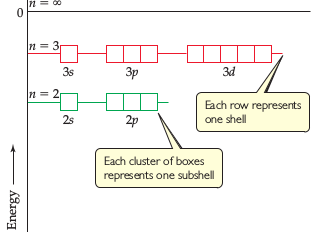
\includegraphics[width=0.4\textwidth]{electron_diagram.png}
\end{figure}
\begin{compactdesc}
\item[Electrons positioned] by using a probability distribution which depends on
    their energy level.
\item[Line spectrum]
\item[Spectral lines of Hydrogen] energy must be absorbed to emit an electron.
    Wavelength of each spectra line:
    \[
        \lambda = R_H(1/n_1^2 - 1/n_2^2)
    \]
\item[Energy of hydrogen emissions]
    \[
        \Delta E = -2.18*10^{-18}J \big(1/n_f^2 -n_i^2 \big)
    \]
\item[Orbital diagram] visualization of each $e^-$'s quantum numbers in an
    atom or molecule. Row of boxes, one box holds at most a pair of arrows
    pointing in opposite directions ($e^-$) and groups of boxes are slightly
    separated to indicate different orbitals p, s, d, f.
\item[Electron Quantum Numbers] $n, l, m_l, m_s$
\item[Energy level] $n \in N^+$
\item[Orbitals] p, s, d, f $l \in 0\dots n - 1$
\item[Magnetic quantum number] a box, $m_s \in -l \dots l$
\item[Spin magnetic quantum number] up/down, $m_l = \pm 1/2$
\item[Subshell] electrons share $n, l$
\item[Pauli's exclusion principle] all $e^-$ in an atom have unique quantum
    numbers.
\item[Hund's rule] the preferred $e^-$ arrangement has maximum $e^-$ with the
    same spin $m_s$
\end{compactdesc}

\begin{figure}[H]
    \centering
    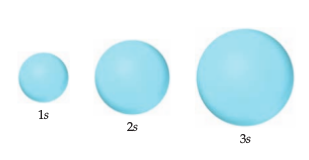
\includegraphics[width=0.2\textwidth]{s_orbital.png}
    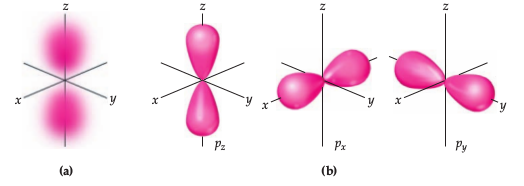
\includegraphics[width=0.3\textwidth]{p_orbitals.png}
    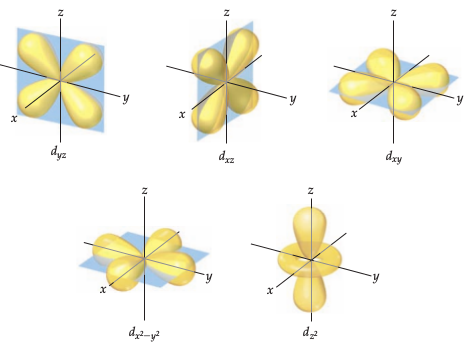
\includegraphics[width=0.3\textwidth]{d_orbitals.png}
\end{figure}

\end{multicols}
\end{mdframed}




\section{Chapter 7. Periodic Properties of the Elements}

\secttoc

{\footnotesize
\begin{multicols}{3}
\begin{compactenum}
    \item Explain effective nuclear charge $Z_{eff}$
    \item Trends in atomic/ionic radii, ionization energy, electron affinity
    \item Radius change on loss or gain of $e^-$
    \item Electron configuration of ions
    \item Change in ionization energy as $e^-$ are added or removed, especially
        core electrons
    \item Irregulairites in periodic table, electron affinity and configuration
    \item Differences in metals and nonmetals (basicity of metal oxides,
        acidity of nonmetal oxides)
    \item Correlate atomic properties with electorn configuration
    \item Balanced equations for reactions of groups 1A and 2A with water,
        oxygen, hydrogen and halogens
    \item Unique properties of hydrogen
    \item Atomic properties of groups 6A 7A and 8A with chemical reactivity
        and physical properties
\end{compactenum}
\end{multicols}
}



\begin{mdframed}
\subsection{Periodic Properties of the Elements}
\begin{multicols}{2}
\begin{compactdesc}
\item[Effective nuclear charge] $Z_{eff}$ roughly equal to $Z - S =$ number of
    protons - number of nonvalence $e^-$. The 1s orbital acts as a
    ``lampshade'' to the 2s, 2p orbitals, and so on\dots \textbf{Trend:} increases to
    the right.
\item[Ionization energy] It becomes harder to remove successive $e^-$.
    I = \ce{X (g) -> X^+ (g) + e^-}.
    I$_2$ = \ce{X^+ (g) -> X^{2+} (g) + e^-}.
    \textbf{Trend:} increases to the top-right.
\item[Electron Affinity] Energy for reaction \ce{X (g) + e^- -> X^- (g)}.
    If positive, ions are unstable. \textbf{Trend:} increases to the top-right.
    \ce{F} and \ce{Cl} have the highest.
\item[Atomic radius] Cations are smaller, anions are larger. \textbf{Trend:} increases
    to the bottom-left.
\item[Isoelectric series radius] same charge ions? Size decreases as atomic
    number increases: $\ce{O^{2-}} > \ce{Br^-} > \ce{F^-} > \ce{Al^{3+}}$
\item[$e^-$ configuration of ions] Add or remove $e^-$ from the highest n,
    then l.
\end{compactdesc}
\end{multicols}
\end{mdframed}




\begin{mdframed}
\subsection{Metals}
\begin{multicols}{2}

\begin{compactdesc}
\item[Trend:] metallic character increases to the bottom-left.
\item[Shiny] silver
\item[Malleable and ductile] can be hammered into sheets and stretched into
    wires
\item[Compounds] usually ionic
\item[Solid conductors] of both heat and electricity
\item[Only one liquid] at room temperature: \ce{Hg}
\item[Form cations] in aqueous solution, tend to make basic solutions.
\item[Low first] ionization energy $I_1$
\item[Common reactions]
 \[\ce{oxide + H2O -> hydroxide}   \]
 \[\ce{oxide + acid -> salt + H2O} \]
\end{compactdesc}

\subsection{Alkali metals}
\begin{compactdesc}
\item[Soft solids] naturally present only in compounds
\item[Good conductors]
\item[Low] densities, melting points
\item[Very] reactive, colorful flames when burned
\item[Common reactions]
    \[\ce{2M (s) + H2 (g) -> 2MH (s) }\]
    \[\ce{2M (s) + S (s) -> M2S (s) }\]
    Vigorous reaction in water:
    \[\ce{2M(s) + 2H2O(l) -> 2MOH(aq) + H2(g)}\]
\item[Special with Oxygen] can coerce oxygen to form peroxide: \ce{2Na + 2O -> Na2O2}
    or super peroxide: \ce{K + O2 -> KO2}
\end{compactdesc}

\subsection{Alkaline metals}
\begin{compactdesc}
\item[Solid] release colorful flame when burned
\item[Compared to Alkali metals] harder, denser, less reactive
\item[Water reactions] Be inert; Mg slowly, faster with steam; all others react
    slowly with water
\item[Tend to lose] their two outer $s$ $e^-$.
\end{compactdesc}

\end{multicols}
\end{mdframed}


Metalloids in between.


\begin{mdframed}
\subsection{Nonmetals}
\begin{multicols}{2}
\begin{compactdesc}
\item[Many colors] but no luster
\item[Usually brittle]
\item[Poor conductors] heat and electricity
\item[Nonmetal oxides] molecules. Form acidic solutions.
\item[High first] ionization energy $I_1$
\item[Common reactions]
    \[\ce{oxide + H2O -> acid} \]
    \[\ce{oxide + base -> salt + H2O} \]
\end{compactdesc}

\subsection{Noble Gases}
\begin{compactdesc}
\item[Monatomic] almost no reactions
\item[Filled] s and p orbitals
\item[Possible compounds] exist in rare, laboratory conditions
    \ce{XeF_{2/4/6}}, \ce{KrF2}, \ce{HArF}
\end{compactdesc}



\subsection{Hydrogen}
\begin{compactdesc}
\item[Resembles a] nonmetal more than an Alkali.
\item[Preserves] $e^-$, tends to covalent bonds
\item[Most stable] \ce{H2(g)}
\item[Proton] \ce{H+} present in water
\end{compactdesc}


\subsection{Oxygen group}
\begin{compactdesc}
\item[Atypical nonmetals]
\item[Oxygen stable as] \ce{O2}
\item[Peroxide] \ce{O2^-}
\item[Superperoxide] \ce{O2^{2-}}
\item[Sulfur stable as] \ce{S8}
\item[Stability of water-like] $\ce{H2O} > \ce{H2S} > \ce{H2Se} > \ce{H2Te}$
\item[Possible reaction] air pollutant:
    \[\ce{S(s) + O2(g) -> SO2 (g)}\]
\end{compactdesc}



\subsection{Halogens}
\begin{compactdesc}
\item[Typical] nonmetals
\item[Very] soluble, negative $e^-$ affinity
\item[Fluoride] is extremely reactive
\item[Diatomic] molecules formed such as \ce{I2}, \ce{Cl2}, except F
\item[Trend:] melting, boiling points increase as elements get heavier
\item[Common reactions]
    \[\ce{H2(g) + X2 -> 2HX (g)}\]
    \[\ce{Cl2(g) + H2O(l) -> HCl(aq) + HOCl(aq)}\]
\end{compactdesc}


\end{multicols}
\end{mdframed}





\section{Chapter 8. Basic Concepts of Chemical Bonding}

\secttoc

{\footnotesize
\begin{multicols}{3}
\begin{compactenum}
    \item Lewis symbols for atoms and ions
    \item Lattice energy. Rank based on ion sizes and charges.
    \item $e^-$ config and octet rule to draw Lewis structure
    \item Electronegativity differences and non-polar/polar covalent and ionic
        bonds
    \item Charge separation in diatomic molecules based on dipole moment
        and bond length
    \item Formal charges, ID dominant Lewis structures
    \item Recognize molecules where resonance structures are needed, draw
        dominant res. struct.
    \item All exceptions to octet rule
    \item Relationship between bond type (single, double, triple),
        bond strength/enthalpy, and bond length
    \item Bond enthalpies to estimate enthalpy changes for gas-phase reactants
        and products
\end{compactenum}
\end{multicols}
}

\begin{mdframed}
\subsection{Lewis Structures}
\begin{multicols}{2}
\begin{compactdesc}
\item[Representation] of electron arrangement and bonds. Valence $e^-$ are
    drawn as dots around atom, shared pairs are lines between atoms.
    Most atoms require 8 valence $e^-$, H needs 2.
\item[Electron Config of Ions] remove or add $e^-$ to highest n, then l.
\item[Formal Charge] valence - $\frac{1}{2}$bonding - non-bonding
\item[Most common Lewis structure] has the lowest formal charge
\item[Not enough valence] electrons could cause a multiple bond.
\end{compactdesc}

\subsection{Resonance structures}
The actual bonds of a substance with multiple valid bonding schemes cannot be
modeled using a single Lewis structure. Examples, Benzene and \ce{O3}:
\begin{figure}[H]
    \centering
    
\includegraphics[width=0.24\textwidth]{benzene.png}
    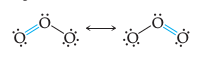
\includegraphics[width=0.24\textwidth]{ozone.png}
\end{figure}


Benzene's arrangement confers special stability to molecules.

\subsection{Exceptions to the Octet Rule}
\begin{compactdesc}
\item[Odd number of $e^-$] \ce{BF3} has resonance and six valence around Boron,
    \ce{NO} has 11 valence electrons
\item[Hypervalent] molecule or ion has more than an octet around central atom
    Only period 3++, due to larger size.
\item[Octet gives unfavorable] distribution.
\item[Large atom] surrounded by large number of small electronegative atoms,
    enough to overpower the octet rule.
\item[Electron configuration] shows distribution of $e^-$ in orbitals.
    $\ce{F}: [\ce{He}] 2s^2 2p^5$
\end{compactdesc}

\begin{figure}[H]
    \centering
    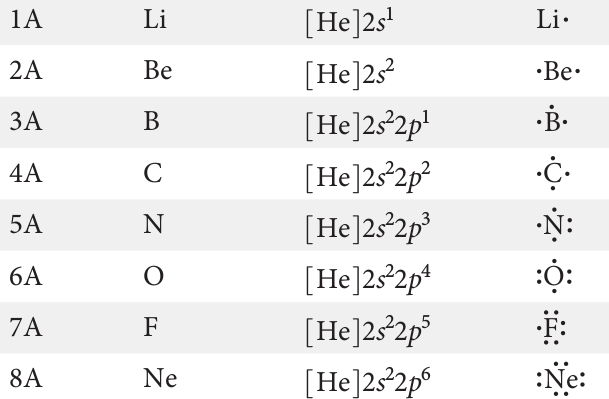
\includegraphics[width=0.3\textwidth]{lewis_basics.png}
\end{figure}

\end{multicols}
\end{mdframed}



\begin{mdframed}
\begin{multicols}{2}
\subsection{Ionic Bonds}
\begin{compactdesc}
\item[Lattice energy] indicates energy needed to separate an ionic substance
    into its gaseous components: \ce{AB -> A+ (g) + B^- (g)}
\item[Related] to Coulomb's law for particles.
\item[Born-Haber cycle]
    Used to calculate the elusive lattice energy using several known energies
    and Hess's law.
\end{compactdesc}




\subsection{Strengths and Lengths of Covalent Bonds}
\begin{compactdesc}
\item[Strength] is determined by energy needed to break the bond
\item[Bond enthalpy] $\Delta H$ needed to break a bond in one mole of a gaseous
    substance: \ce{Cl2(g) -> 2Cl(g)}. Represented as D(\ce{Cl-Cl})
\item[Enthalpies of Reactions] can be determined using bond enthalpies, even
    if $\Delta H_f^\circ$ are not known for all involved.
    Imagine two steps: energy to break all bonds as needed, energy to form new
    bonds.
\item[Bond length] decreases with increasing number of bonds between two atoms.
\item[Smaller bond length] larger $\Delta H$
\end{compactdesc}

\begin{figure}[H]
    \centering
    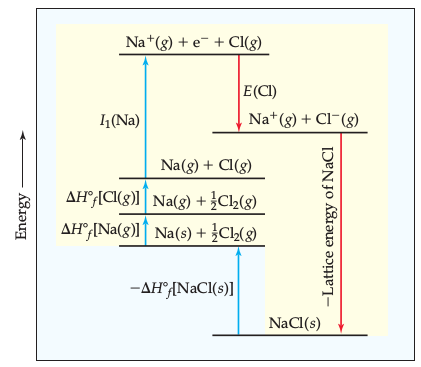
\includegraphics[width=0.4\textwidth]{Born_Haber_cycle.png}
\end{figure}

\end{multicols}
\end{mdframed}


\begin{mdframed}
\subsection{Bond Polarity and Electronegativity}
\begin{multicols}{2}
\begin{compactdesc}
\item[Electronegativity] ability of an atom in a molecule to attract $e^-$.
    Based on ionization energy, electron afinity and other properties.
    \textbf{Trend:} increases to the top-right
\item[Bond polarity] equality of $e^-$ distribution in covalent bond
\item[Nonpolar covalent] equal electron sharing. Difference in
    e.neg = 0.
\item[Polar covalent] not equal electron sharing. Partial charge represented
    as $\delta +$ and $\delta -$. In HF, H has partial positive, in \ce{H2O}
    H has partial negative. Difference in e.neg about 0.5.
\item[Ionic bonds] very unequal electron sharing. Difference in e.neg $\gg 0.5$.
\item[Dipole moment] indicates direction and magnitude of partial charge.
    Relates to charge and radius: $\mu = Q \cdot r$.
\end{compactdesc}

\begin{figure}[H]
    \centering
    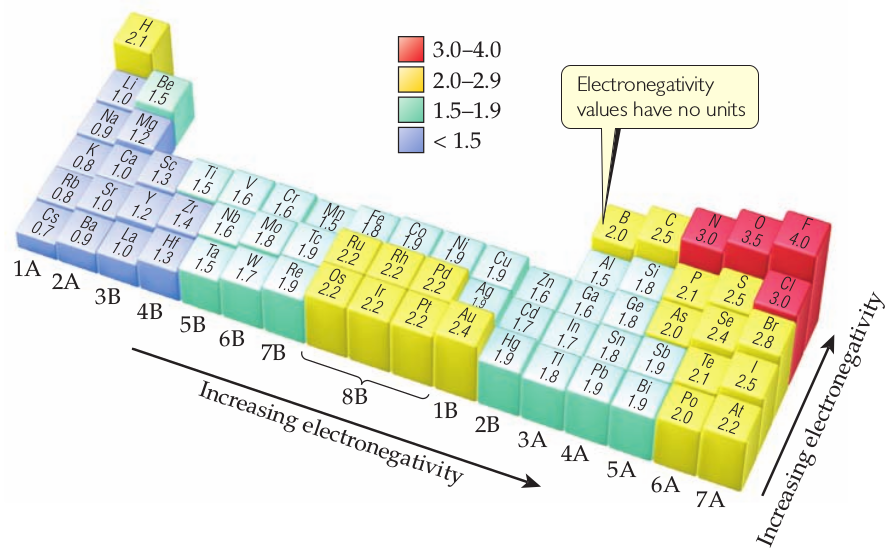
\includegraphics[width=0.5\textwidth]{electronegativity_table.png}
\end{figure}
\end{multicols}
\end{mdframed}


\section{Chapter 9. Molecular Geometry and Bonding Theories}

\secttoc

{\footnotesize
\begin{multicols}{3}
\begin{compactenum}
    \item Predict 3D shapes using VSEPR model
    \item Polar or nonpolar based on geometry and individual dipole moments
    \item Orbital overlap and covalent bonds
    \item Hybridization atoms in molecules based on molec structures
    \item Overlap and $\sigma, \pi$ bonds.
    \item Delocalized $\pi$ bonds in molecules like Benzene
    \item Count $e^-$ in delocalized $\pi$ system
    \item Concept of bonding and antibonding MOs and draw examples of $\sigma$
        and $\pi$ MOs.
    \item MO energy-level diagram. Place $e^-$ to obtain bond orders and $e^-$
        configurations of diatomic molecules.
    \item Correlate bond order, bond strength/enthalpy, bond length,
        magnetic properties with MO descriptions of molecules.
\end{compactenum}
\end{multicols}
}

\begin{mdframed}

\subsection{Molecular Shapes}
\begin{figure}[H]
\centering
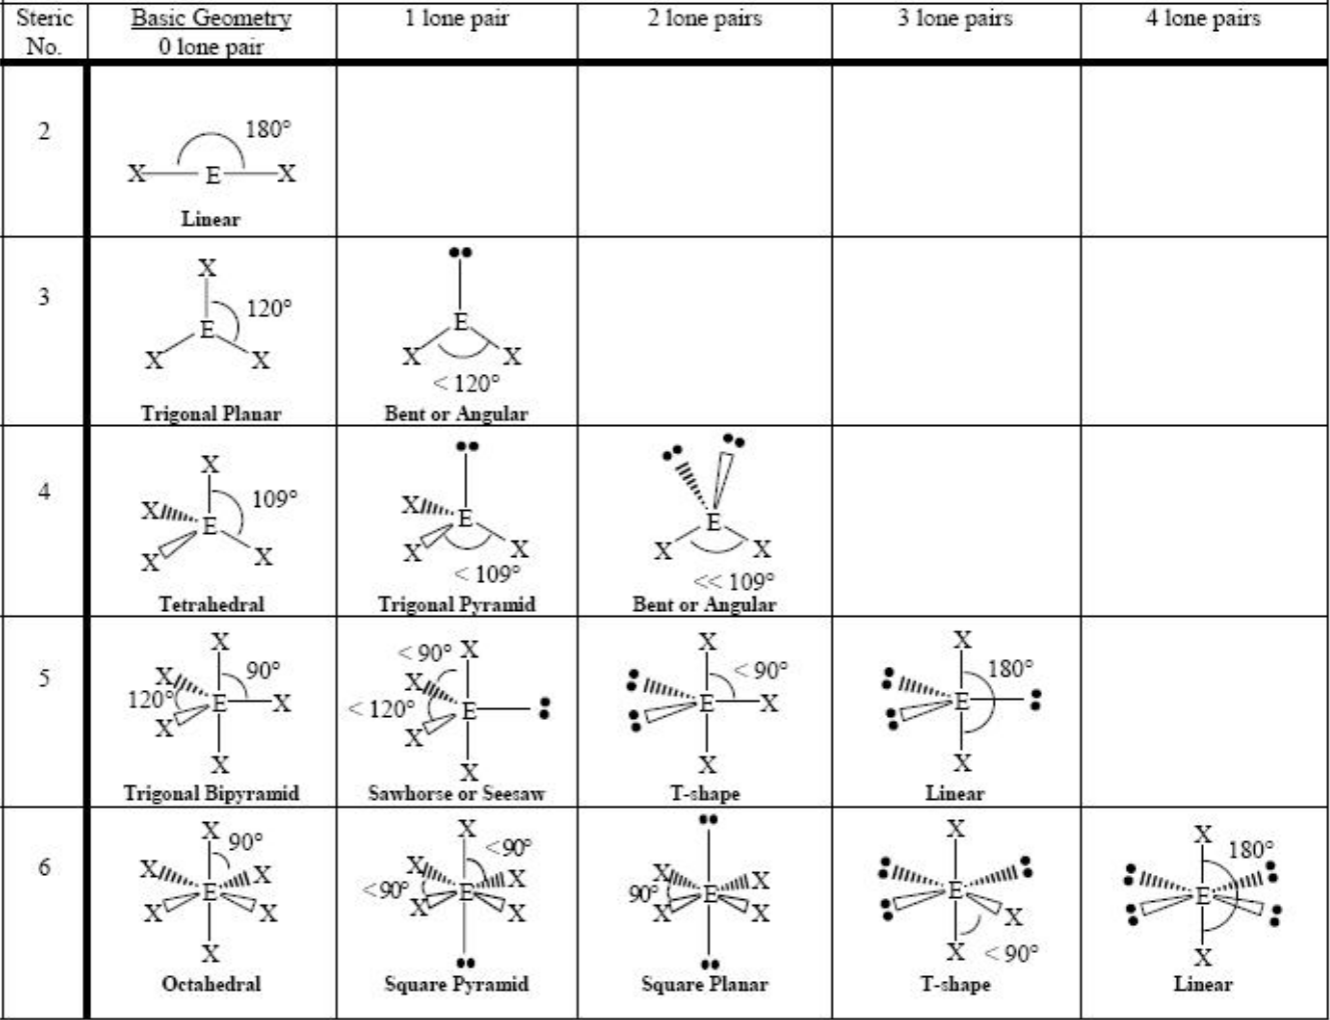
\includegraphics[width=\textwidth]{molecule_shapes.png}
\end{figure}

\subsection{VSEPR Model}
\begin{multicols}{2}
\begin{compactdesc}
\item[Shapes minimize] electron repulsion
\item[Electron Domain] a bonding pair, a multiple bond, or a non-bonding
    $e^-$. \ce{CCl2O} has 3 domains about the central atom.
\item[Nonbonding] takes up more space
\item[Multiple centers?] just find the shape for each center
\item[For 6 domains:] octahedral arrangement is the stablest
\end{compactdesc}


\end{multicols}
\end{mdframed}




\begin{mdframed}
\subsection{Covalent Bonding, Orbital Overlap}
\begin{multicols}{2}
\begin{compactdesc}
\item[Overall Polarity] of a covalent molecule. Consider the shape and each
    dipole, they may cnacel each other out, if they don't then the molecule is
    indeed polar.
\item[Combining VSEPR with Lewis] structures suggests covalent bonds form by
    the intersection of two non-bonding orbitals.
\end{compactdesc}
\begin{figure}[H]
\centering
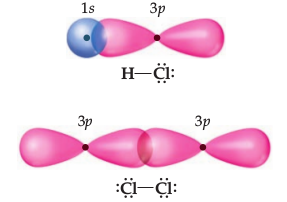
\includegraphics[width=0.3\textwidth]{orbital_overlap.png}
\end{figure}

\end{multicols}



\end{mdframed}




\begin{mdframed}
\subsection{Hybrid Orbitals}
\begin{multicols}{2}
\begin{compactdesc}
\item[Hybrid orbitals] combined atomic orbitals, have different shapes
\item[Hybridization] mixing orbitals, although number of orbitals must remain
    constant.
\item[Hypervalent] central atoms aren't generally hybridized.
\item[Linear $180^\circ$] arrangement of domains implies $sp$ hybridization.
\item[Triangular $120^\circ$] arrangement implies $sp^2$ hybridization, total 3.
\item[Tetrahedral $109.5^\circ$] arrangement implies $sp^3$ hybridization, total 4.
\item[Not all orbitals] need $s$ contact, can also be non-bonding, \ce{NH3},
    \ce{H2O} have $sp^3$ orbitals.
\item[To find] draw Lewis structure, find shapes, any $s$ orbitals? Must be
    hybrid.
\end{compactdesc}
\end{multicols}
\begin{figure}[H]
\centering
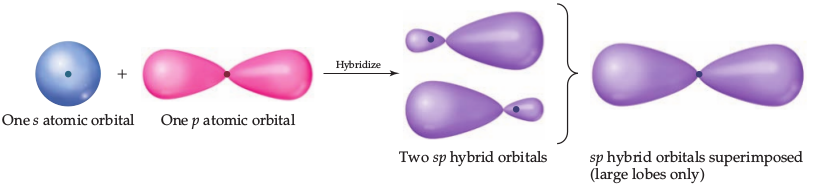
\includegraphics[width=0.9\textwidth]{sp_orbital.png}
\end{figure}

\end{mdframed}




\begin{mdframed}
\begin{multicols}{2}
\subsection{Multiple Bonds}
\begin{compactdesc}
\item[Single bonds] are called $\sigma$. Always local.
\item[Triple and double bonds] have one $\sigma$ and two or one $\pi$ bonds.
    Weaker -- roundabout for $e^-$ -- but reduces rotation.
\item[p$_\pi$ orbital] is the un-hybridized $2p$ orbital in an $sp^2$ that can
    be involved in forming a $\pi$ orbital.
\item[Benzene] rigid thanks to the \textbf{delocalized} (floating) $e^-$ in
    double bonds.
\end{compactdesc}
\begin{figure}[H]
\centering
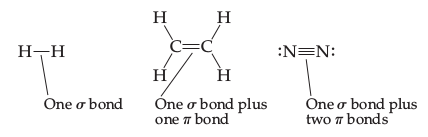
\includegraphics[width=0.4\textwidth]{sigma_pi_bonds2.png}
\end{figure}
\begin{figure}[H]
\centering
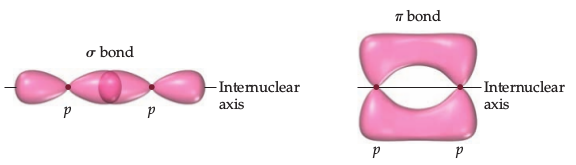
\includegraphics[width=0.45\textwidth]{sigma_pi_bonds.png}
\end{figure}
\begin{figure}[H]
\centering
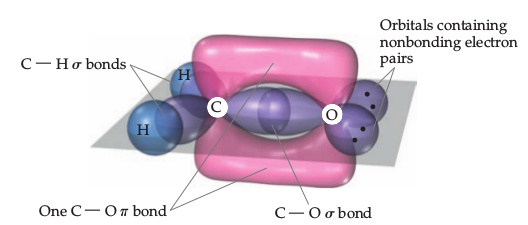
\includegraphics[width=0.45\textwidth]{h2co_orbitals.png}
\end{figure}

\end{multicols}
\end{mdframed}




\begin{mdframed}
\begin{multicols}{2}
\subsection{Molecular Orbitals}
\begin{compactdesc}
\item[Molecular orbital] wave functions describing $e^-$. Orbitals combine to
    cover the whole molecule. MO can have 0, 1 or 2 $e^-$
\item[Number of MO] number of atomic orbitals combining to make MOs.
\item[Bonding MO] waves add constructively to form mighty bond
\item[Anti-Bonding MO] waves add destructively, $e^-$ repelled.
\item[Bond order] $\frac{1}{2}$ (bonding $e^-$ - anti-bonding $e^-$).
\item[Trend:] as bond order increases, bond enthalpy increases and bond
    distance decreases
\item[Electrons arranged] according to Hund's Rule and Pauli's E. Principle.
\item[Core electrons] do not contribute to molecular bonding much
\end{compactdesc}



\subsection{Period 2 Diatomic Molecules}
\begin{compactdesc}
\item[Homonuclear diatomic] molecules (two identical)
    \begin{compactenum}
    \item number of MO = number of AO combined
    \item AO most effectively combined with other AO of similar energy
    \item Effectiveness of combo relates to overlap.
    \item MO can have two $e^-$ with opposite spin (Pauli)
    \item Hund's rule obeyed for same energy MOs
    \end{compactenum}
\item[Heteronuclear diatomic] similar to homo-nuclear, but an MO has a greater
    contribution from AO to which it is closer in energy. \ce{NO}:
    $\sigma_{2s}$ is closer to the O $2s$ than to the N $2s$, thus
    the sigma has greater contribution from O than N.
\item[Paramagnetism] unpaired $e^-$ cause magnetic attraction
\item[Diamagnetism] no unpaired $e^-$ weak magnetic repulsion
\end{compactdesc}
\end{multicols}
\end{mdframed}

\begin{mdframed}
\begin{multicols}{2}
\begin{figure}[H]
\centering
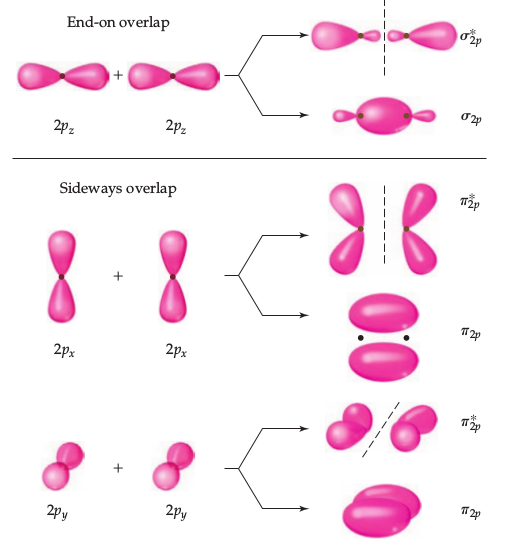
\includegraphics[width=0.45\textwidth]{2p_orbital_overlap.png}
\end{figure}


\begin{figure}[H]
\centering
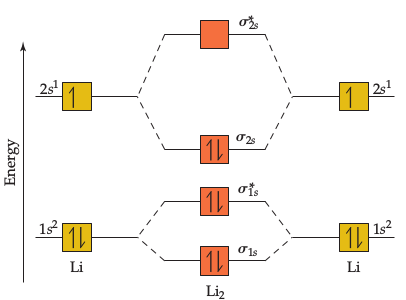
\includegraphics[width=0.40\textwidth]{li2_energy_level_diagrams.png}
\end{figure}
\begin{figure}[H]
\centering
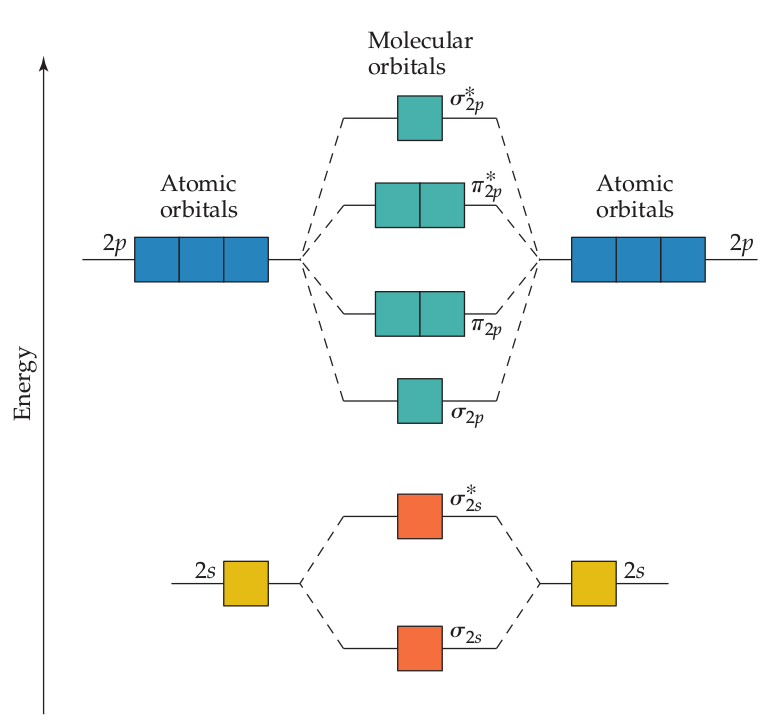
\includegraphics[width=0.45\textwidth]{period2_energy_level_diagrams.png}
\end{figure}
\begin{figure}[H]
\centering
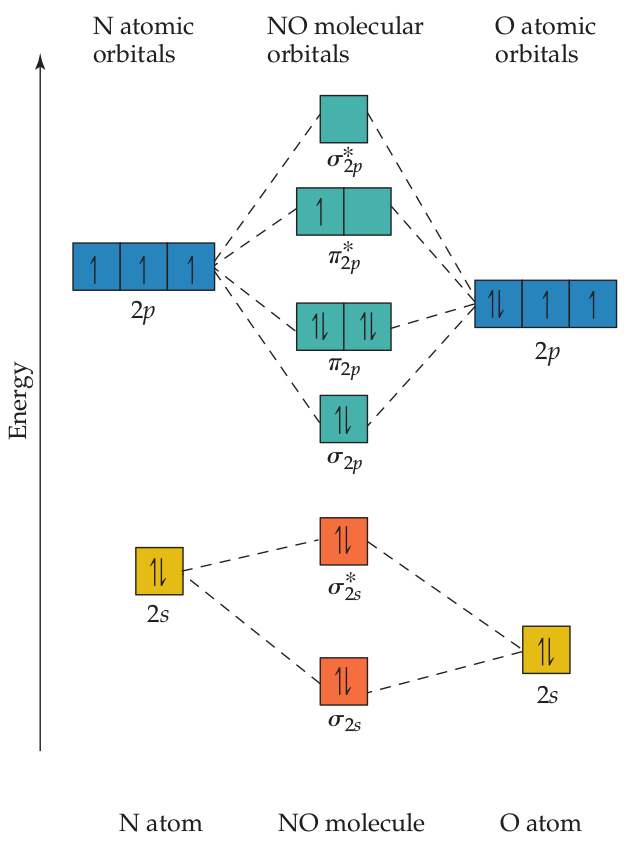
\includegraphics[width=0.45\textwidth]{no_energy_level_diagrams.png}
\end{figure}
\end{multicols}
\begin{figure}[H]
\centering
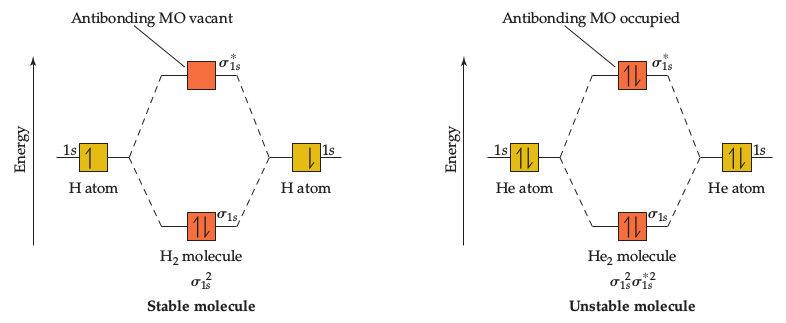
\includegraphics[width=0.8\textwidth]{h2_he2_energy_level_diagrams.png}
\end{figure}
\end{mdframed}






% Among the dead were 16 teenagers and two teachers from a German high school who had just completed a week-long exchange program in Spain. Two German opera singers also died in the crash, as did a pair of newlyweds who'd just married on Saturday. Three Americans—Yvonne Selke, 58, and her daughter, Emily Selke, 22 (pictured above); the third victim was identified by the State Department as Robert Oliver—were on board, as were citizens from Argentina, Morocco, Spain, Germany, Australia, Britain, Iran, Colombia, Kazakhstan, the Netherlands, Israel, and Japan.

\section{Chapter 10. Gases}

{\footnotesize
\begin{multicols}{3}
\begin{compactenum}
    \item Convert between pressure units, mostly torr and atm
    \item Calculate P, V, n, or T
    \item Explain how gas laws relate to ideal-gas equation
    \item Density or MW of a gas
    \item Volume of gas consumed/formed
    \item Total pressure of a gas mixture given partial pressures
    \item Kinetic molecular theory of gases: gas laws, rates of effusion/diffusion
    \item Explain why volumes, intermolecular attractions cause gases deviate
        from ideal gas laws
\end{compactenum}
\end{multicols}
}

\begin{mdframed}
\begin{multicols}{2}
\begin{compactdesc}
    \item[Units] 1 atm = 760 torr = 1.0132 $\cdot10^5$ Pascals
    \item[Charles' law] $V/T$ is constant
    \item[Boyle's law] $PV$ is constant
    \item[Ideal gas law] $PV = nRT$ where $R = 0.08205 \frac{Latm}{molK}$
    \item[Van der Waal's equation] for non-ideal gases, some corrections
        must be made.
        $a, b$ are gas specific. Larger gas molecules are less ideal.
        \[
            \Big(P + \frac{n^2a}{V^2} \Big)(V - nb) = nRT
        \]
    \item[RMS speed] of molecules $\sqrt \frac{3RT}{M}$
    \item[Rate of effusion] lighter gases effuse faster
        $\frac{r_1}{r_2} = \sqrt \frac{M_2}{M_1}$.
    \item[Density of a gas] $\frac{PM}{RT}$
    \item[Partial pressure] $p_\text{total} = \sum_\text{each gas} p$
    \item[Mole fraction] $X = \frac{P_1}{P_t} = \frac{n_1}{n_t}$ moles of gas
        and total moles, total pressure and partial pressure.
        $P_1 = \frac{n_1}{n_2} P_t = X_1 P_t$.
\end{compactdesc}
\end{multicols}
\end{mdframed}

\section{Chapter 11. Liquids and IMFs}

\secttoc

{\footnotesize
\begin{multicols}{3}
\begin{compactenum}
    \item IMFs: dispersion, dipole-dipole, hydrogen bonding, ion-dipole
    \item Explain polarizability, relate to dispersion forces
    \item Explain viscosity, surface tension, capillary action
    \item Names of state changes, exo or endo thermic?
    \item Interpret heating curves, get enthalpy changes (temp/phase)
    \item Critical pressure, crit temperature, vapor pressure,
        normal boiling/melting points, critical point, triple point
    \item Sketch phase diagrams, water's = special
    \item Molecular arrangements and characteristics of nematic, smectic,
        cholerestic liquid crystals. Features of those that favor liquid
        crystalline phases
\end{compactenum}
\end{multicols}
}

\begin{mdframed}
\subsection{Liquids}
\begin{compactdesc}
\item[]
\item[Viscosity] ease of molecule motion relative to each other.
    \textbf{Trend:} decreases with size.
\item[Surface tension] net inward force that must be countered to expand the surface
    area of a liquid.
\item[Cohesive forces] molecules bind to each other
\item[Adhesive forces] bind to surface
\item[Capillary action] rise of liquid up narrow tubes
\item[Heat of sublimation] energy needed to move solid directly to gas phase.
    Equal to $\Delta H_{fus} + \Delta H_{vap}$.
\item[Vapor pressure] pressure exerted by the substance's vapor above the
    surface of a liquid. There's always some vaporization.
\item[Volatile] evaporate readily
\item[Boiling point] vapor pressure = external pressure. Molecules can break
    free of their neighbors
\end{compactdesc}

\begin{figure}[H]
\centering
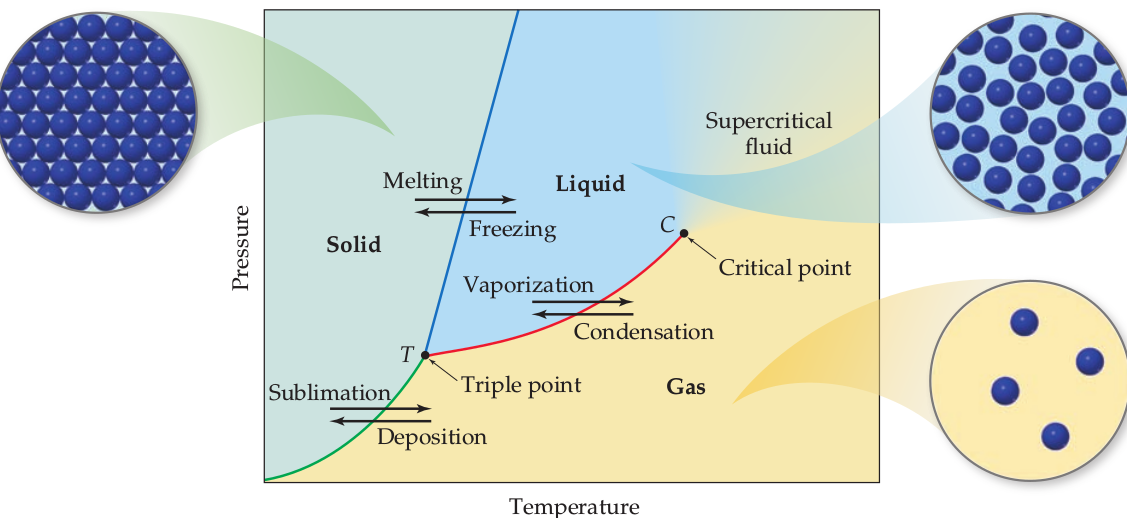
\includegraphics[width=0.75\textwidth]{phase_diagram.png}
\end{figure}

\begin{figure}[H]
\centering
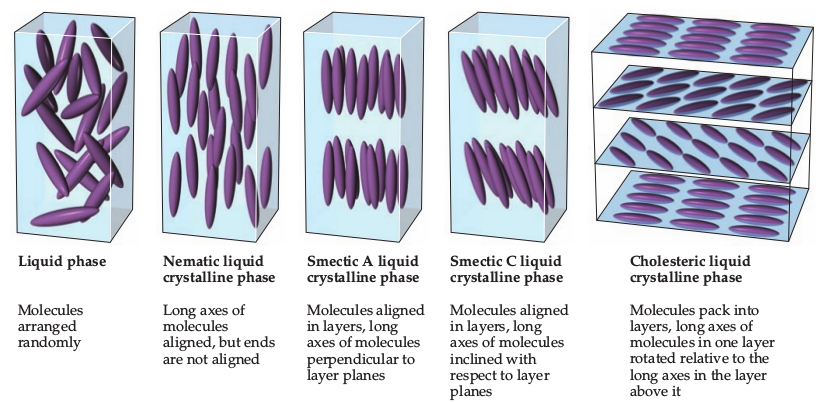
\includegraphics[width=\textwidth]{liquid_crystals.png}
\end{figure}


\end{mdframed}


\begin{mdframed}
\subsection{Intermolecular Forces}
Stronger IMFs mean higher viscosity, surface tension (maintain surface area)
and capillary action.
For molecules of approximately equal mass and size, \textbf{the strength of
intermolecular attractions increases with increasing polarity}.

\begin{tabularx}{\linewidth}{>{\bfseries}l l X X}
    Name & strength & description & \\
    \midrule
    Dispersion & weakest & instantaneous $e^-$ imbalance disrupt neighbors
        & all molecules do it, oblong, heavier = stronger \\
    Dipole-dipole & weak & between dipoles
        & only between polar molecules \\
    Van der Waal's & weak group & includes dispersion, dipole-dipole. Short range
        & repulsive/attractive, stronger = higher BP\\
    Hydrogen bonding & strong & 10\% covalent, mostly electrostatic
        & molecules with \ce{NH}, \ce{OH}, \ce{HF} groups \\
    Ion-dipole & strongest & between polar group and ion
        & example: \ce{H2O} and an ion \\
\end{tabularx}
\end{mdframed}

\section{Chapter 12. Solids}

\secttoc

{
\footnotesize
\begin{multicols}{3}
    \begin{compactenum}
    \item classify solids based on bonding/IMFs
    \item differences between crystalline and amorphous solids
        (crystal lattice, unit cells, etc)
    \item why are there a limited number of lattices? 5 2D and 7 3D
        primitive lattices
    \item characteristics/properties of metals
    \item empirical formula and density of ionic/metallic solid given a unit cell.\
        estimate length of a cubic unit cell from radii of atoms present
    \item homogeneous/heterogeneous alloys
    \item electron-sea model of metallic bonding
    \item MO model of metallic bonding to generate electronic band structure
        of metals, qualitatively predict MP \& BP, hardness
    \item predict structures of ionic solids given radii and empirical formula
    \item MP \& BP in terms of IMF and crystalline forces
    \item valence/conduction bands. band gap, holes, semiconductor and insulator
    \item account for relative band gap energies of semiconductors through periodic trends
    \item n-type and p-type doping to control conductivity
    \item plastic, thermoplastic, thermosetting plastic, elastomer, copolymers,
        and cross-linking
    \item polymers formed from monomers, what features allow this?
    \item polymer chain interactions impact physical properties
    \item properties of semicond. and metals change with nanometer crystals
    \item structure/properties of fullerenes, carbon nanotubes and graphene
    \end{compactenum}
\end{multicols}
}

\begin{mdframed}
    \subsection{Classification}
    \begin{multicols}{3}
\begin{compactdesc}
    \item[Types of kinetic energy] translational, rotational, vibrational.
        \item[solids] lowest energy phase, mostly vibrational energy
        Atoms packed tight. It is surfaces of solids that react.
        \item[metallic solids] held together by delocalized sea of valence $e^-$
        \item[ionic solids] mutual attraction between anions/cations
        \item[covalent-network solids] extended network of covalent bonds
        \item[molecular solids] weak IMFs
        \item[polymers] long chains of atoms, covalent
        \item[nanomaterials] individual crystals are 1-100nm.
    \end{compactdesc}
\end{multicols}
\end{mdframed}


\begin{mdframed}
    \subsection{Structures}

    \begin{multicols}{3}
\begin{compactdesc}
        \item[crystalline solids] regularly repeating pattern, usually flat
            faces, specific angles
        \item[amorphous solids] no long-range order
        \item[unit cell] smallest repeating unit
        \item[crystal lattice] geometrical pattern of points where unit cells go.
            \emph{N-dimensional} lattices
            can be defined with \emph{n} vectors
        \item[motif,]group of atoms, associated with each \emph{lattice point}
        \item[primitives] 5 2D lattices, 7 3D lattices
        \item[square  ] $a = b, \gamma = 90$
        \item[rect    ] $a \neq b, \gamma = 90$
        \item[hex     ] $a = b, \gamma = 120$
        \item[rhombic ] $a = b$
        \item[oblique ] $a \neq b$
        \item[cubic] $a = b = c, \alpha = \beta = \gamma = 90$
        \item[tetra] $a = b \neq c, \alpha = \beta = \gamma = 90$
        \item[hexa] $a = b \neq c, \alpha = \beta = 90, \gamma = 120$
        \item[rhombohedral] $a = b \neq c, \alpha = \beta = \gamma \neq 90$
        \item[orthorhombic] $a \neq b \neq c, \alpha = \beta = \gamma = 90$
        \item[monoclinic] $a \neq b \neq c, \alpha = \beta = 90, \gamma \neq 90$
        \item[triclinic] $a \neq b \neq c, \alpha \neq \beta \neq \gamma$
        \item[body-centered cubic] additional point at center of such a cell
        \item[face-centered] additional points at the faces of a cell
    \end{compactdesc}
\end{multicols}
\end{mdframed}

\begin{mdframed}
    \subsection{Metallic solids}

    \begin{multicols}{3}
\begin{compactdesc}

    \item[Metallic solids] good conductors of electricity and heat, malleable (sheets), ductile (wires)
    \item[Structure] usually simple, just need one atom on each
        lattice point.
    \item[Primitive] 1 atom per unit cell. \textbf{Body-centered} 2 atoms per.
        \textbf{Face-centered} 4 atoms per.

    \item[Tight packing] is favorable if $e^-$ are shared.
        \textbf{Hexagonal close packing} hcp, \textbf{Cubic} ccp.
    \item[Coordination number] 12 for hcp and ccp. In both,
        each sphere has 12 equidistant neighbors. Any immediate neighbors.

    \item[Alloy] material that contains more than one element and behaves like
        a metal.
    \item[Substitutional alloy] two metallic components have similar radii and
        bonding characteristics. Less typical if radii differ $>15\%$.
    \item[Interstitial alloy] solute atoms must have smaller bonding radii
        than solvent. Extra bonds mean stronger/harder/less ductile.
    \item[Heterogeneous alloy] components are not dispersed uniformly.
        Properties depend on both composition and the manner in which the solid
        was formed from molten mixture (ex: cooled fast/slow?).
    \item[Inter-metallic compounds] not mixtures. Definite properties.

\end{compactdesc}
\end{multicols}
\end{mdframed}



\begin{mdframed}
\subsection{Metallic bonding}

\begin{multicols}{2}
\begin{compactdesc}
    \item[Electron-sea model] metal = array of metal cations in a sea of
        valence electrons. Electrons migrate to positive end. Also, their
        motion facilitates transfer of kinetic energy (heat).
        Not enough $e^-$ on each atom, must share!
    \item[Molecular-orbit model, Band Structure]
        Orbitals shared by entire metal. Fills low \ce{->} high.
        Bands are per-molecule in nonmetals. 3d band, 4s, 4d bands \dots
    \item[Conduction band] easy to remove $e^-$ from here, the top.
    \item[Valence band] $e^-$ stick to here, closest to nucleus.
    \item[Stronger bonds] mean higher boiling/melting points, heats of fusion,
        hardness, and so forth.
    \item[Group 6B] middle, highest strength. More does not always mean more
        strength, repulsion in antibonding MOs can ruin it. Recall bond order
        $\frac{1}{2}$ (bonding $-$ antibonding $e^-$)
\end{compactdesc}
\end{multicols}

\begin{figure}[H]
    \centering
    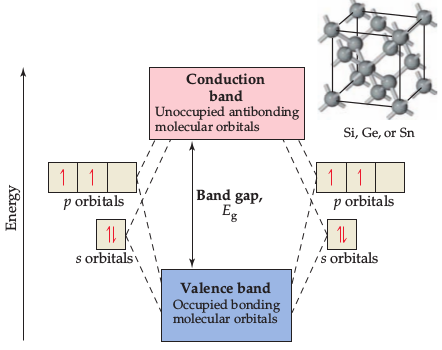
\includegraphics[width=0.5\textwidth]{band_gap.png}
\end{figure}

\end{mdframed}



\begin{mdframed}
\subsection{Complex}

\begin{multicols}{2}
\begin{compactdesc}
\item[Color] caused by $e^{-}$ shuffling about the d-orbital. \ce{TiO2} has
    no electrons in the d-orbital and is colorless.
\end{compactdesc}
\end{multicols}
\end{mdframed}




\begin{mdframed}
    \subsection{Ionic solids}

    \begin{multicols}{3}
\begin{compactdesc}
    \item[Ionic solids] electrostatic attraction between cations and anions.
        Interactions increase as charges of ions increases (lattice energy++).
    \item[Structures] cations are usually much smaller than anions.
    \item[Coordination number] smaller than metals.
        Close packing is prohibited by repulsive forces.
    \item[Formula from structure]
        $\frac
            {\text{Cations per formula unit}}
            {\text{anions per formula unit}}
        $  is equal to
        $ \frac
            {\text{anion coord number}}
            {\text{cation coord number}} $
    \item[No conduction] as solids! Molten salt can conduct.
    \end{compactdesc}
\end{multicols}
\end{mdframed}



\begin{mdframed}
\begin{multicols}{3}

    \subsection{Molecular solids}

\begin{compactdesc}
    \item[Molecular solids] atoms/neutral molecules held by dipole-dipole,
        dispersion, and/or hydrogen bonds.
    \item[Weak bonds] low BP, MP (below 200 Celsius), soft.
        More symmetry means tighter packing, stronger bonds.
\end{compactdesc}

    \subsection{Covalent-network solids}

\begin{compactdesc}
    \item[Strong bonds] covalent bonds beat IMFs. Diamond, quartz.
\end{compactdesc}

    \subsection{Semiconductors}

\begin{compactdesc}
    \item[Semiconductors] harder for $e^-$ to move between levels because of a
        ``band gap'' separating valence/conduction bands.
        Typically group 4 (C, Si, Ge, Sn). Band gap + +, conduction - -
    \item[large band gap] no conduction!
\end{compactdesc}


\end{multicols}
\end{mdframed}



\begin{mdframed}
    \subsection{Polymers}

\begin{multicols}{3}
\begin{compactdesc}
\item[Polymers] chains or branched structures composed of monomers.
\item[Addition Polymerization] two monomers added to each other, double bond
    between is elimintated.
\item[Condensation Polymerization] condensing two monomers together, getting
    rid of intermediate small molecule once they are linked.
\item[Chain inititaion] a free radical initiator possesing an unstable
    unpaired electron attacks a monomer unit to cause it to expose another
    unstable $e^{-}$.
\item[Chain propogation] this unit attacks other monomers, forming an ever
    growing chain.
\item[Polymer crosslinks] produce harder substances with less flexibility.
\item[Commercial example] polyethylene chains contain between $10^3$ and
    $10^5$ \ce{CH2} units.
\end{compactdesc}
\end{multicols}
\end{mdframed}



% \begin{mdframed}
%     \subsection{Nanomaterials}
%
% \begin{multicols}{3}
% \begin{compactdesc}
% LOW-PRIORITY
% \end{compactdesc}
% \end{multicols}
% \end{mdframed}


\section{Chapter 13. Properties of Solutions}


\secttoc

{\footnotesize
\begin{multicols}{3}
\begin{compactenum}
    \item Enthalpy/entropy changes affect solution formation
    \item IMFs and solubility, like dissolves like
    \item Equilibrium in the solution process, solubility of a solute
    \item Temperature and solid, liquid or gas solubility
    \item Partial pressure of a gas and its solubility
    \item Molarity, molality, mole fraction, percent composition, ppm, inter-convert!
    \item Colligative property? How do non-electrolytes and electrolytes affect?
    \item Vapor pressure of a solvent over soln
    \item BP elevation, FP depression
    \item Osmotic pressure of a solution
    \item Solution vs colloid
    \item Similarities between motions of gas molecules and the motions of
        colloids in a liquid
\end{compactenum}
\end{multicols}
}

\begin{mdframed}\subsection{Solution Process}
\begin{multicols}{2}\begin{compactdesc}
    \item[Natural tendency] formation of solutions is favored by the increase in
        entropy that accompanies mixing.
    \item[Intermolecular interactions] solute-solute, solvent-solvent,
        solvent-solute. The first two must be defeated to disperse and make room.
    \item[Solvation] when ions/molecules of solute are split and surrounded by
        solvent.
    \item[Solvation] solute is surrounded by solvent molecules.
    \item[Hydration] solvation with water as solvent
    \item[Energy cost] Solute and solvent must break down, then they must be
        mixed.
        $ \Delta H_{soln}
        = \Delta H_{solute} + \Delta H_{solvent} + \Delta H_{mix}$

        Think:
            \ce{solute$_n$ <=> $n$ solute} takes $\Delta H_{solute}$
            \ce{solvent$_m$ <=> $m$ solvent} takes $\Delta H_{solvent}$
            \ce{$n$ solute + $m$ solvent <=> solution} takes $\Delta H_{mix}$
    \item[Exothermic] $\Delta H_{mix} < 0$
    \item[Endothermic] $\Delta H_{solvent/solute} > 0$ need energy.
    \item[Spontaneity] If overall exothermic, solvation occurs spontaneously.
        Explains why \textbf{likes dissolve likes}. Similar IMFs have similar
        costs.
\end{compactdesc}\end{multicols}\end{mdframed}


\begin{mdframed}\subsection{Saturated solutions and solubility}
\begin{multicols}{2}\begin{compactdesc}
    \item[Equilibrium] \ce{solute + solvent <=> solution}
    \item[Crystallization] when solute is reverted to original state.
        ``Undissolved.'' Happens at the same time as solvation. Visible when
        solvent is spent and cannot maintain solvation interactions with enough
        solute.
    \item[Saturation] Equilibrium with undissolved solute. Additional solute
        will not dissolve (unless you add heat!). \textbf{Make a super-saturated: }
        add heat, lower heat, creates unstable solution.
    \item[Solubility] how much solute an amount of solvent can dissolve.
\end{compactdesc}\end{multicols}\end{mdframed}


\begin{mdframed}\subsection{Factors affecting solubility}
\begin{multicols}{2}\begin{compactdesc}
    \item[Like dissolves like] the stronger the interactions between solvent
        and solute, the greater the solubility. Polar dissolves polar; non-polar,
        non-polar.
    \item[Miscible] liquids that mix in all proportions. May be
        \textbf{immiscible.}
    \item[Pressure] liquid and solid solubilities are unaffected. Gas solubility
        is related to its partial pressure above liquid.
    \item[Henry's law] molarity of gas $=$ constant $\cdot$ partial pressure
        $S_g = k P_g$. Constant $k$ depends on temperature, solute and solvent.
    \item[Temperature] increase  increases solubility of most \textbf{solids}
        in water. There are exceptions \ce{Ce2 (S O4)3}
    \item[Temperature] increase decreases solubility of most \textbf{gases}
        in water
\end{compactdesc}\end{multicols}\end{mdframed}


\begin{mdframed}\subsection{Expressing solution concentrations}
\begin{multicols}{2}\begin{compactdesc}
    \item[Mass percentage]
        $\frac {\text{mass of component in soln}}
               {\text{total soln mass}} \cdot 100\% $
    \item[Parts per million/billion] $ \frac{mg}{kg} $, also
        $\frac {\text{mass of component in soln}}
               {\text{total soln mass}} \cdot 10^6 $
    \item[Mole fraction]
        $\frac {\text{moles of component in soln}}
               {\text{total moles}} $
    \item[Molality] Commonly used, independent of temperature!
        $\frac {\text{moles of solute}}
               {\text{kg of solvent}} $, little m.
    \item[Molarity]
        $\frac {\text{moles of solute}}
               {\text{litres of soln}} $, big M.
\end{compactdesc}\end{multicols}\end{mdframed}


\begin{mdframed}\subsection{Colligative Properties}
\begin{multicols}{2}\begin{compactdesc}
    \item[Colligative property] depend on concentration of solute, type of
        solvent. Not on the type of solute.
    \item[Raoult's law, vapor pressure depression]
        Applies to \emph{nonvolatile solute}
        \[
            P_\text{solution} = X_\text{solvent} P_\text{solvent}
        \]
        \[
            \Delta P = X_\text{solute} P_\text{solvent}
        \]
        \[
            X_\text{y} = \frac{\text{moles of y}}{\text{total moles}}
        \]
    \item[Solutions w/ two or more volatile] components, the vapor pressure of
        the solution is the sum of the vapor pressure of each component as
        calculated by Raoult's law.
    \item[Ideal solution] obey Raoult's law. Solute-solute, solvent-solvent and
        solute-solvent interactions all equal.
    \item[Molal boiling point elevation constant] BP of a solution is
        higher than that of the solvent. $m$ is molality.
        \[
            \Delta T_b = T_{b(\text{solution})} - T_{b(\text{solvent})}
            = i K_b m
        \]
    \item[Molal freezing point depression constant] FP of a solution is lower
        than that of the solvent. $m$ is molality.
        \[
            \Delta T_f = T_{f(\text{solution})} - T_{f(\text{solvent})}
            = - i K_f m
        \]
    \item[van't Hoff Factor] number of fragments a solute breaks up into for
        that particular solvent. Usually anion/cation dissociated.
    \item[True van't Hoff Factor] $i = \frac
        {\Delta T_f \text{measured}}
        {\Delta T_f \text{theoretical}}$
    \item[Osmosis] Solvent molecules pass through semipermeable membrane
        between two solutions of differing concentration. Solvent always
        goes to solution with lower solvent concentration. Want equilibrium
        (isotonic). Hypotonic: lower osmotic pressure, hypertonic: more
        concentrated.
    \item[Osmotic pressure] $\Pi = i \big( \frac{n}{V_\text{soln}} \big) RT
                                 = iM_\text{molarity}RT$
\end{compactdesc}\end{multicols}\end{mdframed}


\begin{mdframed}\subsection{Colloids}
\begin{multicols}{2}

    Some mixtures appear to initially dissolve, but gravity separates solute
    from solvent.
    \begin{compactdesc}
    \item[Colloids] between homogeneous mixtures and true solutions. Large
        solvent molecules/particles.
    \item[Tyndall effect] Large enough to \textbf{scatter light}, Tyndall
        effect.
    \item[Hydrophilic] folds to keep hydrophobic groups away from water.
        Polar groups go to surface. Usually have \ce{N} or \ce{O} and a charge.
    \item[Hydrophobic] can only be dispersed if stabilized. Otherwise, they
        run away. One method is via adsorption of ions to the surface. This
        repels particles from each other and causes interactions with the water.
    \item[Emulsion] a suspension of one liquid in another, like Milk.
    \item[Adsorption] think adhesion. Sticking stuff to surface.
    \item[Brownian motion] collisions cause colloid particles to exhibit random
        motion
\end{compactdesc}\end{multicols}\end{mdframed}




\section{Chapter 14. Chemical kinetics}


\secttoc

{\footnotesize
\begin{multicols}{3}
\begin{compactenum}
    \item Factors affecting rate of reactions
    \item Rate of reaction given time and concentration
    \item Relate rates of product formation and reactant disappearance given
        balanced chemical equation
    \item Explain form and meaning of a rate law (reaction order, rate constant)
    \item Determine these given measure rates for various concentrations
    \item Integrate rate laws
    \item Relationship between rate constant of 1st order and half-life
    \item Activation energy affects a rate, Arrhenius equation
    \item Predict rate law for a multi-step mechanism given each step.
    \item Explain principles of catalysis
\end{compactenum}
\end{multicols}
}

\begin{mdframed}\subsection{Reaction Rates}
\begin{multicols}{2}
\begin{compactdesc}
    \item[Chemical kinetics] concerned with rates of reaction
    \item[Reaction rates] affected by physical states
        the more readily collisions occur, the more rapidly goes the reaction.
        Affected by reaction concentrations and temperature. Catalysts increase
        reaction rates by affecting activation rates.
    \item[homogeneous] same phase
    \item[heterogeneous] different phases
\end{compactdesc}
\end{multicols}
\end{mdframed}


\begin{mdframed}\subsection{Rates and Concentration}
\begin{multicols}{2}
    Rate is typically measured in molarity per second, change in
    concentration, ($M/s$).
\begin{compactdesc}
    \item[Average rate] of disappearance of A $=
        \frac{\Delta [\text{A}]}{\Delta t}$
    \item[Instantaneous rate] concentrations can be measured using \textbf{spectroscopy}.
    \item[Beer's law] concentration, c is directly proportional to absorbance, A.
        $A = \epsilon b c$, b is path length.
    \item[Stoichiometry] In reaction \ce{A -> B} the rate of appearance of product
        is the rate of disappearance of reactant.
    \item[Relative rates] In reaction \ce{aA + bB -> cC + dD}, the rates are
        $   -\frac{1}{a}\frac{\Delta A}{\Delta t}
          = -\frac{1}{b}\frac{\Delta B}{\Delta t}
          =  \frac{1}{c}\frac{\Delta C}{\Delta t}
          =  \frac{1}{d}\frac{\Delta D}{\Delta t}
        $. This does not hold true if intermediate substances are formed in
        significant amounts.
    \item[Rates are positive] by convention

    \item[(Differential) Rate Law] Typically of form $R = -k[A]^m[B]^n$
    \item[Rate constant] $k :: M^{-m - n + 1}s^{-1}$. Different for every reaction
        and temperature; $>10^9$ means fast, $<10$ means slow.
    \item[Reaction orders]
        $m, n$ usually 0, 1, 2. Can be negative or fractional.
    \item[Overall reaction order] $n + m$
    \item[Rate law from Initial rates]
        \(
            n = \frac {\ln \frac {Rate_1} {Rate_2} } {\ln \frac {[A]_1} {[A]_2} }
        \)
\end{compactdesc}
\end{multicols}
\end{mdframed}



\begin{mdframed}
\subsection{Concentration and Time}
\begin{multicols}{2}
    Integrated, linear rate laws for the first order reaction \ce{A -> \dots}
\begin{compactdesc}
    \item[First-order reaction]
        $\ln [A]_t = \ln [A]_0 - kt$.
    \item[Second order reaction]
        $\frac{1}{[A]_t} = \frac {1} {[A]_0} + kt$.
    \item[Zero-order reaction] $[A]_t = [A]_0 - kt$
    \item[Half life] of a first-order depends only on $k$. $t_{1/2} = -\frac{\ln 1/2} {k}$
\end{compactdesc}
\end{multicols}
\end{mdframed}





\begin{mdframed}\subsection{The Effect of Temperature on Rates}
\begin{multicols}{2}
\begin{compactdesc}
    \item[Collision model] based on kinetic molecular theory. Molecules
        must collide to react, so goes the theory. More energy/temp means
        more collisions, faster rate. Molecules must be aligned correctly on impact.
    \item[Activation energy, $E_a$] needs to be achieved.
        Must also be moving fast enough and in the correct orientation.
        Lower $E_a$ means faster reactions.
        Never negative.
    \item[Rate does not depend on] $\Delta H$, only on $E_a$
    \item[Activated complex/transition state] Enough energy in the right
        direction, now the molecules may react together.
        Highest potential energy. It's all downhill from here!
    \item[Arrhenius equation] Rate constant incorporates all of these:
        $k = Ae^{-E_a / RT}$. A is the \textbf{frequency factor}, constant as
        temperature is varied. Can be used to find different $k$s.
        $R = 8.314 J \cdot mol^{-1} \cdot K^{-1} $
        $= 0.082057L \cdot atm \cdot K^{-1}\cdot mol^{-1}$
    \item[Solve for $k$] at different temperatures. $A$ and $E_a$ remain
        constant:
        \[
            \ln \frac{k_1}{k_2} = \frac{E_a}{A} \big( 1/T_2 - 1/T_1 \big)
        \]
\end{compactdesc}
\end{multicols}
\end{mdframed}



\begin{mdframed}\subsection{Reaction Mechanisms}
\begin{multicols}{2}
\begin{compactdesc}
    \item[Reaction mechanism] Steps which constitute a reaction.
        Order in which bonds are modified. And change in relative positions.
    \item[Elementary reactions] Single step. Defined by \# of molecules
        colliding: \textbf{uni/bi/ter}molecular.
        $>3$ molecules colliding is improbable.
    \item[Intermediate]
        \ce{NO2 + CO -> NO + CO2} is actually
        \ce{NO2 + NO2 -> NO3 + NO} then \ce{NO3 + CO -> NO2 + CO2}
        Together: \ce{2NO2 + NO3 + CO -> NO2 + NO3 + NO + CO2}
        Thus \ce{NO3} is an intermediate, common in both sides of the addition.
        Multi-step reactions have one or more such substances.
    \item[Rate laws] of elementary reactions have an overall reaction order
        equal to the number of molecules involved. Termolecular, $n + m = 3$.
        A single chemical equation cannot tell us if a reaction is elementary!
    \item[Rate-determining step] is the slowest. If initial, likely that its
        rate law will govern that of the overall.
    \item[Slow initial step] the rate is usually equal to the rate of the
        initial step.
\end{compactdesc}

If the initial step is fast, the rate law may be derived by assuming
equilibrium and solving the $k_1$ and $k_{-1}$ to get rid of the intermediate
substance \ce{NOBr2}.

Example: \[\ce{2NO + Br2 -> 2NOBr}\] could be a termolecular reaction, or
the fast equilibrium step and a slow final step
\[\ce{NO + Br2 <=>T[k1][k-1] NOBr2}\]
\[\ce{NOBr2 + NO ->T[k2] 2NOBr}\]
$k_1, k_{-1}$ reach
equilibrium meaning rate of (forward = reverse) and the total rate constant
$k = k_2 \frac{k_1}{k_{-1}}$. Two steps, but only uni/bi molecular is more likely.
35 or more steps are sometimes derived!
\end{multicols}
\end{mdframed}



\begin{mdframed}\subsection{Catalysts}
\begin{multicols}{2}
\begin{compactdesc}
    \item[Catalyst] changes the speed of (initial) activation of a reaction without being changed itself
        Usually done by lowering $E_a$. Opposite = inhibitor.
    \item[Homogeneous catalyst] same phase as reactants. Not so for a
        \textbf{Heterogeneous catalyst} (first step usually adsorption of
        reactants)
    \item[Adsorption] (think adhesion), how fast a substance is bound to a
        surface.
    \item[Enzymes] marvelously efficient biological catalysts. Usually huge
        proteins, kilo to mega amu. Very selective. Faster than nonbiologicals,
        $10^3 - 10^7$ reactions per molecule per second (turnover number).
    \item[Substrates] substances reacting at the active site
    \item[Active site] location of catalysis.
    \item[Lock-and-key model] Explanation for specificity of an enzyme.
\end{compactdesc}
\end{multicols}
\end{mdframed}

\section{Chapter 15. Chemical equilibrium}


\secttoc

{\footnotesize
\begin{multicols}{3}
\begin{compactenum}
    \item What is meant by equilibrium, relate to rates
    \item Write equilibrium-constant expression for any reaction
    \item Inter-convert $K_c$ and $K_p$
    \item Magnitude of equilibrium constant and relative amounts of reactants
        and products
    \item Manipulate constant to reflect changes in chemical equation
    \item Heterogeneous reaction equilibrium constant (EC)
    \item Calculate EC from concentration measurements
    \item Predict direction of a reaction given EC and conc.s
    \item Calculate concentrations given EC and one equi. conc.
    \item Calculate equi. conc.s given EC and starting conc.s
    \item Le Ch\^{a}telier's principle to predict how conc.s, volume or temperature
        of system at equilibrium affects the equilibrium position
\end{compactenum}
\end{multicols}
}

\begin{mdframed}
\begin{multicols}{2}
\subsection{Rock bottom}
\begin{compactdesc}
    \item[Dynamic equilibrium] two opposing events have the same rate, no net
        change occurs.
    \item[Vapor pressure] rate of molecules leaving the liquid near the surface
        is equal to the rate of their return to liquid state
    \item[Chemical equilibrium] opposing reactions with the same rate.
    \item[Example] \ce{N2O4 (g) (colorless) <=> 2NO2 (g) (brown)}. The
        equilibrium constant is \[
            k = \frac{k_f}{k_r} = \frac{[\ce{NO2}]^2}{[\ce{N2O4}]}
        \]
    \item[At equilibrium] concentrations do not change and products/reactants
        cannot escape system.
    \item[For equilibrium] to occur, both reactions must be able to occur.
\end{compactdesc}
\end{multicols}
\end{mdframed}


\begin{mdframed}
\begin{multicols}{2}
\subsection{Equilibrium constant}
\begin{compactdesc}
    \item[Unique to an equilibrium] even if initial concentrations change
    \item[law of mass action] consider the general equilibrium
        equation \ce{aA + bB <=> dD + eE}. The equilibrium expression is
        \[
            K_c = \frac { [\ce{D}]^d [\ce{E}]^e} {[\ce{A}]^a [\ce{B}]^b }
        \]
    \item[No units] $k_c$ is unitless because another method of measuring it
        ends up unitless.
    \item[Activity] of a substance in an ideal mixture is the ratio of $C$ or
        $P$ to a reference like $1M$ or $1atm$. $A = C M / 1 M$ thus, no units
    \item[Solids and Liquids] activity is unity.
    \item[Depends on order] of the equilibrium reaction, even though they
        are naturally order-less. Thus, in a way $K_c = \frac{1}{K_c}$.
    \item[Can use partial pressure] instead of concentrations for gaseous
        reactions.
    \item[Converting] $K_p = K_c (RT)^{\Delta n}$ where $\Delta n = $ moles
        of gaseous product -- moles of gaseous reactant.
\end{compactdesc}
\end{multicols}
\end{mdframed}


\begin{mdframed}
\begin{multicols}{2}
\subsection{Direction and Summation of Equations}
\begin{compactdesc}
    \item[Reaction written backwards] $K_{rev} = \frac{1}{K}$
    \item[Reaction multiplied] by a constant $n$, $K_{n} = K^n$.
    \item[Reactions added] simply multiply all $K$s involved.
        Adding the two equations:
        \[ \ce{aA + bB <=> dD + cC} \] with $K_0$ and
        \[ \ce{cC + fF <=> gG + aA} \] with $K_1$ will give
        \[ \ce{bB + fF <=> dD + gG} \] with $K_0 K_1$.
\end{compactdesc}
\end{multicols}
\end{mdframed}


\begin{mdframed}
\begin{multicols}{2}
\subsection{Heterogeneous Equilibrium}
\begin{compactdesc}
    \item[homogeneous] all involved substances in same phase
    \item[heterogeneous] involved substances in different phases
    \item[liquid or solid] substances have an activity equal to unity.
        Ratio of their mass to volume is constant.
\end{compactdesc}
\end{multicols}
\end{mdframed}


\begin{mdframed}
\begin{multicols}{2}
\subsection{Finding K from initial and equilibrium concentrations}
\begin{compactdesc}
    \item[If initial and final known] then $\Delta conc$ is known.
    \item[If initial and another $\Delta conc$ known] use coefficients in balanced
        reaction to relate change in the known with the current unknown.
    \item[If initial and change known] just add!
    \item[Use an ICE table] Initial, Change in, and Equilibrium
        concentrations.
    \item[Example]
        Key steps: finding change in $conc$ knowing only $\Delta conc_{\ce{HI}} $.
        \[
            \Big( 1.87\cdot 10^{-3} \Big)
            \Big( \frac{ 1 mol \ce{H2} } { 2 mol \ce{HI} } \Big)
            = 0.935\cdot 10^{-3}
        \]
\end{compactdesc}
\end{multicols}
\begin{table}[H]
    \begin{tabular}{lccccc}
        & \ce{H2 (g)} & + & \ce{I2 (g)} & \ce{<=>} & \ce{2HI (g)} \\
        Initial & 1.00$\cdot 10^{-3}$ & & 2.00$\cdot 10^{-3}$ & & $0.00$ \\
        Change  & \textbf{-0.935$\cdot 10^{-3}$} & & \textbf{-0.935$\cdot 10^{-3}$} & & \textbf{+1.87$\cdot 10^{-3}$} \\
        Final   & \textbf{0.065$\cdot 10^{-3}$} & & \textbf{1.065$\cdot 10^{-3}$} & & 1.87$\cdot 10^{-3}$ \\
    \end{tabular}
    \centering
    \end{table}
\end{mdframed}


\begin{mdframed}
\begin{multicols}{2}
\subsection{Applications of K}
\begin{compactdesc}
    \item[Predicting the Direction of Reaction] If $Q < K$ then more products
        will be needed, if $Q > K$ then more reactants needed.
    \item[Reaction quotient] Calculated like $K$, but for concentrations or
        partial pressures at any point in the reaction.
    \item[Calculating equilibrium concentrations] just solve for unknowns using
        known equilibrium concentrations.
\end{compactdesc}
\end{multicols}
\end{mdframed}


\begin{mdframed}
\subsection{Le Ch\^{a}telier's Principle}
\begin{multicols}{2}
\begin{compactdesc}
    \item[Le Ch\^{a}telier's Principle] if equilibrium is disturbed in any way,
        the system will shift its position to counteract. ``le-SHOT-lee-ay.''
    \item[Lies to the right] lots of ``product''
    \item[Lies to the left] lots of ``reactant''
    \item[Concentration of reactants increased] increases concentration of products
    \item[Pressure change] by changing volume, if increased in gaseous equilibrium the system
        will want to minimize the number of moles of gas. Constant temperature.
    \item[Volume change] same as pressure change
    \item[Temperature change] If reaction is endothermic, increasing T
        increases $K$. If reaction is exothermic, increasing T decreases $K$.
    \item[Effects of catalysts] activation energies are lowered,
        but $K$ is not changed. Equilibrium will be reached faster.
\end{compactdesc}
\end{multicols}
\end{mdframed}




\section{Chapter 16. Acid-Base Equilibria}


\secttoc

{\footnotesize
\begin{multicols}{3}
\begin{compactenum}
    \item ID Arrhenius acids and bases
    \item Describe nature of hydrated proton, either \ce{H+ (aq)} or \ce{H3O+ (aq)}
    \item ID Br{\o}nsted-Lowry acids and bases and ID conjugate acid-base pairs
    \item Correlate the strength of an acid to the strength of its conjugate
        base
    \item Equilibrium position of a proton-transfer relates to the strengths of
        acids and bases involved
    \item Auto-ionization of water and explain how [\ce{H3O+}] and [\ce{OH-}] are
        related by $K_W$
    \item Calculate the pH given [\ce{H3O+}] and [\ce{OH-}]
    \item Calculate the pH of a strong acid or base given its concentration
    \item Relate $K_a$ and/or $K_b$ for a weak acid/base and its concentration
        and the pH
    \item Calculate $K_b$ for a weak base given $K_a$ of its conjugate acid and
        vice versa
    \item Predict whether an aqueous solution of a salt will be acidic, basic
        or neutral
    \item Predict the relative strength of a series of acids from their
        molecular structures
    \item ID Lewis acids and bases

\end{compactenum}
\end{multicols}
}


\begin{mdframed}
\begin{multicols}{2}
\subsection{Arrhenius Acids and Bases}
\begin{compactdesc}
    \item[Acid] increases concentration of \ce{H+} ions.
    \item[Bases] increase the concentration of \ce{OH-} ions
    \item[Examples] \ce{HCl (g) -> H+ (aq) + Cl- (aq)}
                 \\ \ce{NaOH -> Na+ (aq) + OH- (aq)}
\end{compactdesc}

\subsection{Br{\o}nsted-Lowry Acids and Bases}
\begin{compactdesc}
    \item[Acid-base reactions] involve the transfer of protons from one
        substance to another
    \item[Acid] donates a proton to another substance
    \item[Base] receives a proton
    \item[Hydronium ion] closer to the reality of aqueous solutions.
    \item[Used interchangeably] \ce{H+ (aq)} and \ce{H3O+ (aq)}
    \item[Water acts like] a Br{\o}nsted-Lowry base when a Br{\o}nsted-Lowry
        acid is dissolved:
        \ce{HA + H2O (l) -> H3O+ (aq) + A- (aq)}.
    \item[Water also acts like] a Br{\o}nsted-Lowry acid when a
        Br{\o}nsted-Lowry base is dissolve:
        \ce{B + H2O (l) -> BH+ (aq) + OH- (aq)}
    \item[Amphoteric] substances can behave as either acids and bases.
        Basic if in the presence of something more acidic, acidic if the other
        is more basic.
    \item[Amphiprotic] Either a proton acceptor or donor. Although an
        amphiprotic species must be amphoteric, the
        converse is not true.
    \item[Amphiprotic] \ce{HCO3^- , HS^-, HPO4^2-, HF, H2O}
    \item[Conjugate acid] every base converts into one. \ce{H3O+} is the c.a.
        of \ce{H2O}
    \item[Conjugate base] every acid converts into one. \ce{OH-} is the c.b.
        of \ce{H2O}
    \item[Relative Strengths of Acids and Bases]
        The stronger the acid/base, the weaker its conjugate base/acid.
        \begin{compactenum}
        \item Strong acid's conjugate base shows negligible basicity
        \item Weak acid's conjugate base is a weak base
        \item Negligibly acidic substance's conjugate is a strong base
        \end{compactenum}
    \item[Leveling effect] Stronger acids react with water to produce
        \ce{H3O+} and stronger bases react to produce \ce{OH-}. These
        are the strongest acids and bases that can exist in water.
    \item[Equilibrium favors] transfer of protons to form weaker acids and
        bases.
\end{compactdesc}

\end{multicols}
\end{mdframed}



\begin{mdframed}
\begin{multicols}{2}
\subsection{Auto-ionization of Water}
\begin{compactdesc}
    \item[Autoionization] \ce{H2O (l) + H2O (l) <=> OH- (aq) + H3O+ (aq)}
    \item[Ion-product constant] the equilibrium constant for water
        $k_w = 1\cdot10^{-14}$ at 25 degrees Celsius.
    \item[Neutral solution] \ce{[H+] = [OH^-]}
\end{compactdesc}

\subsection{pH and pOH Scale}
\begin{compactdesc}
\item[pH] is equal to \ce{-\log_{10}[H+]}
\item[pOH] is equal to \ce{-\log_{10}[OH^-]}
\item[pH + pOH] at 25 degrees Celsius is always 14.
\item[Negative pH] indicates a very strong acid
\item[pH greater than 14] indicates a very strong base
\item[pH may be measured] by detecting trace electric charge
\item[pH depends on] concentration of the acid or base
\end{compactdesc}

\end{multicols}
\end{mdframed}




\begin{mdframed}
\begin{multicols}{2}
\subsection{Strong acids and bases}
\begin{compactdesc}
\item[Most common strong acids] six mono-protic:
    (\ce{HClO3}, \ce{HClO4}, \ce{HCl}), \ce{HBr}, \ce{HI}, \ce{HNO3},
    and one diprotic: \ce{H2SO4} but only with the first proton
\item[Strong:] no equilibrium, balance lies entirely to the right
\item[Most common strong bases] ionic hydroxides of the alkali metals, and
    of the heavier alkaline earth metals (Calcium++). The latter are limited
    in solubility.
\end{compactdesc}
\end{multicols}
\end{mdframed}




\begin{mdframed}
\begin{multicols}{2}
\[k_a k_b = k_w\]

\subsection{Weak Acids and $k_a$}
\begin{compactdesc}
    \item[Equilibrium constant for acids] is called the acid-dissociation
        constant $k_a$. Larger means stronger. Need not be aqueous.
        Example for \ce{HA (aq) <=> H+ (aq) + A^- (aq)}:
        \[ k_a = \frac{\ce{[H+] [A^-]}}{\ce{[HA]}} \]

    \item[Percent ionization for acids] Larger also means stronger.
        \[\frac{\ce{[H+]_{equilibrium}}}{\ce{[HA]_{initial}}}\]
    \item[Polyprotic acids] can undergo more than one dissociation. \ce{H2SO3}
        has two protons to give away. It is always easier to remove the first
        proton.
    \item[p$K_a$] is equal to $-\log_{10} k_a$
\end{compactdesc}

\subsection{Weak Bases and $k_b$}
\begin{compactdesc}
     \item[Equilibrium constant for bases] is called the base-dissociation
        constant $k_b$. Larger means stronger. Only for water based!
        Example for \ce{B (aq) + H2O (l) <=> HB+ (aq) + OH^- (aq)}:
        \[ k_b = \frac{\ce{[BH+][OH^-]}}{\ce{[B]}} \]
    \item[Category One] neutral substances that have an atom with a non-bonding
        pair of electrons that can accept a proton. Most have Nitrogen.
        Includes Ammonia and Amines.
    \item[Amines] at least one \ce{N-H} bond in \ce{NH3} is replaced with
        \ce{N-C}.
    \item[Second category] anions of weak acids. The acid \ce{NaClO} has
        the conjugate base \ce{ClO-}.
    \item[p$K_b$] is equal to $-\log_{10} k_b$
\end{compactdesc}

\end{multicols}
\end{mdframed}




\begin{mdframed}
\begin{multicols}{2}
\subsection{Acid-Base Properties of Salt Solutions}
\begin{compactdesc}
\item[Nearly all salts are strong electrolytes] their acid-base properties
    are due to their cations and anions
\item[Hydrolysis] ions react with water to generate \ce{H+} or \ce{OH-}.
\item[An anion can be considered] the conjugate base of an acid \ce{A^-}.
    If it is not a strong acid, it is a weak acid.
\item[Polyatomic cations with one or more protons] can be considered the
    conjugate acids of weak bases.
\item[The larger the charge on the metal ion] the stronger the interaction
    between ion and oxygen of its hydrating water molecules. Facilitates
    proton transfer.
\item[Combined effect of cation and anion]:
    \begin{compactenum}
    \item Anion and cation don't react with water (both from strong a/b)?
        pH should be neutral. \ce{NaCl}, \ce{Ba(NO3)2}, \ce{RbClO4}
    \item Anion produces hydroxide ions, cation doesn't react (from weak acid, strong base)?
        pH should be basic. \ce{NaClO}, \ce{RbF}, \ce{BaSO3}
    \item Cation produces hydronium ions, anion doesn't react (from weak base, strong acid)?
        pH should be acidic. \ce{NH3NO3}, \ce{AlCl3}, \ce{Fe(NO3)3}
    \item Both anion and cation react in water (both from weak)?
        The pH of the solution depends on the relative abilities of the ions to
        react.
        \ce{NH4ClO}, \ce{Al(CH3COO)3}, \ce{CrF3}
    \end{compactenum}
\end{compactdesc}

\end{multicols}
\end{mdframed}


\begin{mdframed}
\begin{multicols}{2}

\subsection{Acid-Base Behavior and Chemical Structure}
\begin{compactdesc}
    \item[Strength of the \ce{H-A}] bond is the greatest indicator of
        acid strength
    \item[Acid Strength]
        \begin{compactenum}
        \item stronger partial charges on H in H bonds. If non-polar, the bond
            is neither acidic nor basic
        \item bond strength, increases as you move to the left-bottom.
            \ce{HBr} is very strong
        \item The greater the stability of the conjugate base \ce{A^-}, the
            stronger the acid.
        \end{compactenum}
    \item[Binary acids] bond strength decreases and acidity and size increase
        down a group.
    \item[Oxyacids] \ce{O-H} bonds present, but the compound is an acid
    \item[OH bond: acid or base] as the electro-negativity of Y in \ce{Y-O-H}
        increases, so does the acidity. Electron density is drawn to \ce{Y}
        so the \ce{O-H} bond becomes weaker and more polar. Also, the stability
        of the conjugate base (\ce{YO^-})increases with the electro-negativity
        of \ce{Y}.
    \item[Acid strength increases] as additional electronegative atoms bond to
        the central atom Y. \[
        \ce{HClO4}
        >
        \ce{HClO3}
        >
        \ce{HClO2}
        >
        \ce{HClO}
        \]
    \item[Carboxylic Acids]
        Contain the carboxyl group \ce{COOH} \chemfig{C ([:90]=O^{-})-O-H}.
        Largest group of organic acids. The conjugate base is stabilized
        by resonance between the two oxygens, spreads negative charge. Also the
        non \ce{O-H} oxygen draws electron density from the broken bond,
        increases polarity.
    \item[Carboxylic acid examples] \ce{CH3COOH}, Benzoic acid
        (benzene and carboxyl), Formic acid \ce{HCOOH}.
\end{compactdesc}
\end{multicols}
\end{mdframed}



\begin{mdframed}
\begin{multicols}{2}
\subsection{Lewis Acids and Bases}
\begin{compactdesc}
    \item[Lewis acids and bases] is a general definition of acids and bases.
    \item[Lewis Acid] electron-pair acceptor
    \item[Lewis Base] electron-pair donor
    \item[Water] is not required. A wider variety of reactions may be treated,
        including acid-base reactions (no proton transfer).
    \item[Strength of electrostatic] interactions
    \item[The interaction of lone pairs] on one molecule with vacant orbitals
        on another is one of the most important concepts in chemistry.
\end{compactdesc}
\end{multicols}
\end{mdframed}








\section{Chapter 17. More Aspects of Aqueous Equilibria}

\secttoc

{\footnotesize \begin{multicols}{3}\begin{compactenum}
\item The Common-ion effect
\item How does a buffer function?
\item Calculate the pH of a buffered solution
\item Same, after adding small amounts of strong acid/base
\item Calculate appropriate quantities to make buffer for certain pH
\item Calculate pH at any point in a strong acid--strong base titration
\item Same, but for weak--strong acid/base or base/acid titration
\item Differences in the prev two titration curves?
\item Estimate $pK_a$ for mono/polyprotic acids form titration curves
\item $K_{sp}$, molar solubility, mass solubility, solve for one
    using two.
\item Molar solubility in presence of common ion
\item Effect of pH on solubility
\item Precipitate when soln.s mixed by comparing $Q$ and $K_{sp}$
\item Ion concentrations needed to begin precipitation
\item Effect of complex-ion formation on solubility
\item Logic of ID of metal ions in aqueous soln by a series of recctions.
\end{compactenum}\end{multicols}}

\begin{mdframed}
\begin{multicols}{2}
\subsection{Common-Ion Effect}
Solution with weak acid/base and a soluble substance containing that acid/base
\textbf{shifts the equilibrium to the left}
concentrations lowering \ce{H+}. Example: adding \ce{CH#COONa (aq)} salt to a
solution of \ce{CH3COOH (aq)} or adding \ce{NH4Cl} electrolyte to solution of
\ce{NH3 (aq)}

\subsection{Buffers}
\begin{compactdesc}
\item[Buffered soluton] small amount of strong acid/base. Resists changes in pH
    by neutralizing any \ce{H+} or \ce{OH^-}.
\item[Composition example] buffer pair \ce{CH3COOH/CH3COO^-}
\item[Composition method 1] mix a weak acid/base with a salt of that acid/base.
    Example: adding \ce{CH3COONa} to soln of \ce{CH3COOH}.
\item[Composition method 2] make conjugate acid/base from weak soln by adding strong
    acid/base. Example: \ce{CH3COOH} and add \ce{NaOH} neutralize half of the
    acetic acid.
\item[Any pH] can be chosen for a buffer
\item[Buffer capacity] how much intruding acid/base can be tolerated without
    straying from \textbf{pH range}
\item[pH Range] usually in range $pK_a \pm 1$.
    Work best when [\ce{HA}] = [\ce{A^-}].
\item[Add \ce{OH^-} ions] acid takes over
    \[\ce{OH^- (aq) + HA (aq) -> H2O(l) + A^-(aq)}\]
\item[Add \ce{H+} ions] base takes over
    \[\ce{H+ (aq) + A^- (aq) -> H2O(l) + HA(aq)}\]
\item[pH of a Buffer]
    Use an ICE table. Cancel out spectator ions. Find [\ce{H+}]
\item[Henderson-Hasselbalch equation] for conjugate acid-base pairs:
    pH $= pK_a + \log\frac{\text{base}}{\text{acid}}$
    where $K_a$ of the acid is used and the two conc.s are at equilibrium
    Can use initial conc.s -- easier -- but use this assumption with care.
    \[[\ce{H+}] = K_a \frac{[\ce{HA}]}{[\ce{A^-}]}\]
\item[Adding a strong acid/base]
    Strong acid/base always neutralized completely with weak base/acid (water's
    $1/k_w = 10^{14}$) To calculate pH of buffer after addition:
    \begin{compactenum}
    \item Find limiting reactant in the acid-base neutralization reaction
        (\ce{OH^-} or \ce{H+} into ICE table)
    \item Use new values of \ce{HA}, \ce{A^-} and $k_a$ to find
        [\ce{H+}]
    \end{compactenum}
    Balance:
    \[\ce{OH^- + HA -> H2O + A^-}\]
    \[\ce{H+ + A^- -> HA}\]
\end{compactdesc}
\begin{figure}[H]
    \centering
    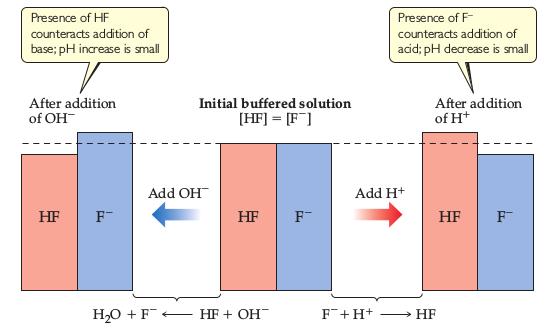
\includegraphics[width=\linewidth]{buffer_action.png}
\end{figure}
\end{multicols}
\end{mdframed}




\begin{mdframed}
\begin{multicols}{2}
\subsection{Acid-Base Titrations}
\begin{compactdesc}
    \item[pH titration curve] indicates pH as the titration progresses.
        See initial, equivalence and post-equivalnce values.
    \item[Equivalence point] moles of acid = moles of base
    \item[Strong base titrates strong acid] pH rises from about 0 to about
        14; equivalence point 7.
    \item[Strong acid titrates strong weak] pH lowers, same as base titrating
        acid.
    \item[Strong titrates weak] sudden change in pH, but equivalence point is
        closer. May not be 7 due to conjugate base/acid. Equivalence point pH increases
        as $k_a$ decreases, closer to titrator's side.
    \item[Acid-base indicator] can be used instead of pH meter. It must have
        an activation range near the equivalence point.
        Phenolphthalein range 8.3 to 10.0, Methyl red ranges from 4.2 to 6.0.
    \item[Polyprotic acids] curve with two equivalence points.
    \item[Half-equivalence point] $pH = pK_a$
\end{compactdesc}

\begin{figure}[H]
    \centering
    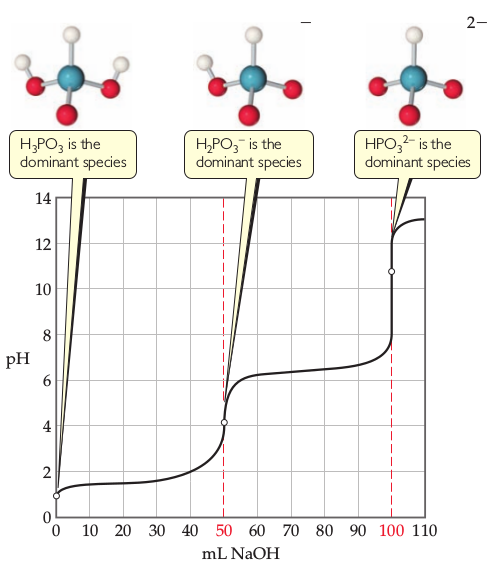
\includegraphics[width=0.8\linewidth]{polyprotic_titration.png}
\end{figure}
\end{multicols}
\end{mdframed}






\begin{mdframed}
\begin{multicols}{2}
\subsection{Solubility Equilibria}
\begin{compactdesc}
\item[Heterogeneous solubility] Species in different phases. Dissolution,
    precipitation of ionic compounds.
\item[Solubility-Product constant] $K_{sp}$ solubility of solid in water.
    $K_{sp} = $ product of concentrations of ions, raised to power of its
    equilibrium coefficient.
    \ce{CaF2} gives $K_{sp} = [\ce{Ca^{2+}}][\ce{F^-}]^2$. Small means
    it doesn't dissolve much.
\item[Solubility] is quantity that dissolves to form saturated soln,
    very volatile.
    $K_{sp}$ measures how much solid dissolves, one for each temperature
    (extreme accuracy? consider concentration).

\item[Solubility from $K_{sp}$] ICE table for dissolved ions, their initial conc.s are 0 unless otherwise noted. Only if no
    other important equilibria affecting solubility.
    Units: $\frac{g}{L \text{ soln}}$, $\frac{mol}{L     \text{ soln}}$.
\item[Deviations] caused by electrostatic between ions, ignoring
    acid-base equilibria, incomplete dissociation (like \ce{MgF+} ions)
\end{compactdesc}
\end{multicols}
\end{mdframed}




%TODO adding OH to soluble salt, ksp problem

\begin{mdframed}
\begin{multicols}{2}
\subsection{Factors affecting solubility}
\begin{compactdesc}
\item[Common-ion effect] generally, solubility of a slightly soluble salt
    decreased by common-ion. Shift left.
\item[pH affects solubility,] increases for basic anions.
    Can dissolve completely in very acidic solution.
    Example: \ce{Mg(OH)2 (s)} usually pH = 10.52 [\ce{Mg^{2+}}] = 0.00017, if
    pH is buffered to 9 and $K_{sp} = 1.8\cdot10^{-11}$ then [\ce{Mg^{2+}}]
    = 0.18M.
\item[Complex ion] very soluble in water. ...
\item[Formation of Complex ions]
\item[Formation constant]
\item[Amphoterism]
\end{compactdesc}
\end{multicols}
\end{mdframed}






\begin{mdframed}
\begin{multicols}{2}
\subsection{Precipitation and Separation of Ions}
\begin{compactdesc}
\item[Q for solubility] $K_{sp}$, but not necessarily at equilibrium.
Can use same as Q in Chapter 15 to find direction of the reaction.
\item[Q $= K_{sp}$] solution is saturated, no precipitate
\item[Q $< K_{sp}$] reaction proceeds to the right, no precipitate
\item[Q $> K_{sp}$] reaction proceeds to the left, precipitate
\item[Selective precipitation] ions can be separated based on solubilities of
    salts. Sulfide ion is commonly used, sulfide salts span wide range.
    CuS $K_{sp} = 6\cdot 10^{-37}$, ZnS $K_{sp} = 2\cdot 10^{-25}$.
    CuS will precipitate with pH around 1, ZnS will precipitate at higher
    pH.
\end{compactdesc}
\end{multicols}
\end{mdframed}






\begin{mdframed}
\begin{multicols}{2}
\subsection{Qualitivative Analysis for Metallic Elements}
\begin{compactdesc}
\item[Metals vary] in their salt solubility, acid-base, complex ions.
    These differences can be used to separate and detect presence of metal
    ions.
\item[Qualitative analysis] presence/absence of species
\item[Quantitative analysis] quantity of species
\item[Common 5 group scheme]
    \begin{compactdesc}
    \item[Group 1] insoluble chlorides, add \ce{HCl}, precipitates
        \ce{AgCl}, \ce{Hg2Cl2}, \ce{PbCl2}
    \item[Group 2] acid-insoluble sulfides, soln. now acidic, \ce{H2S} is
        added, precipitates \ce{CuS}, \ce{Bi2S3}, \ce{CdS}, \ce{PbS},
        \ce{HgS}, \ce{Ag2S3}, \ce{Sb2S3}, \ce{SnS2}. These have low
        $K_{sp}$
    \item[Group 3] base-insoluble sulfides and hydroxides, soln made basic,
        \ce{(NH4)2S} added, precipitates \ce{Al^{3+}}, \ce{Cr^{3+}},
        \ce{Fe^{3+}}, \ce{Zn^{2+}}, \ce{Ni^{2+}}, \ce{Co^{2+}},
        \ce{Mn^{2+}}
    \item[Group 4] insoluble phosphates, \ce{(NH4)2HPO4} precipitates
        \ce{Mg^{2+}}, \ce{Ca^{2+}}, \ce{Sr^{2+}}, \ce{Ba^{2+}}
    \item[Group 5] alkali metal, \ce{NH4+} flame test, other individual tests.
    \end{compactdesc}
\end{compactdesc}

\begin{figure}[H]
    \centering
    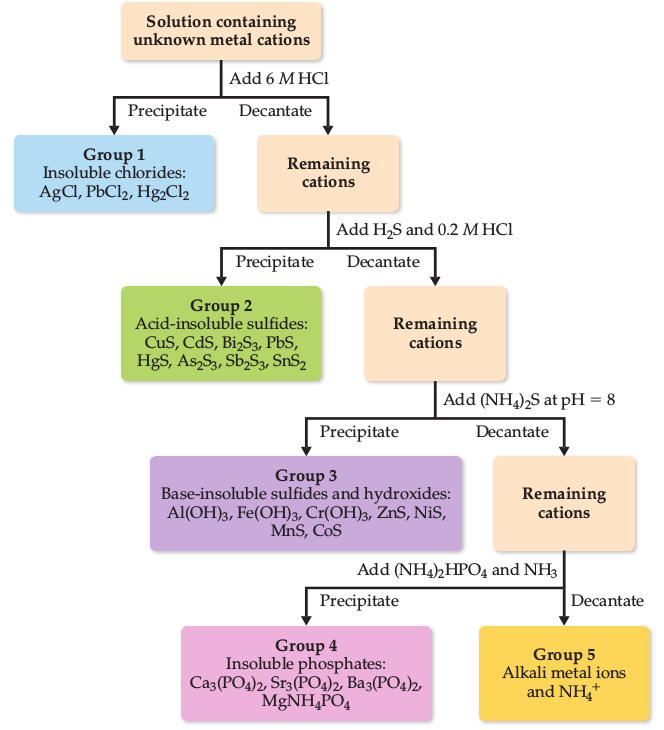
\includegraphics[width=0.9\linewidth]{cation_detection.png}
\end{figure}
\end{multicols}
\end{mdframed}







\setcounter{section}{18}
\section{Chapter 19. Chemical Thermodynamics}
\secttoc

{\footnotesize \begin{multicols}{3}\begin{compactenum}
\item Spontaneous, reversible, irreversible and isothermal processes
\item Entropy and the Second law
\item Entropy and micro-states
\item Possible molecular motions
\item Predict sign of $\Delta$S for physical and chemical
\item The Third law
\item Standard entropy changes using standard molar entropies
\item Entropy changes for an isothermal process
\item Gibbs free energy from enthalpy change
\item Entropy change at a temperature
\item Free-energy changes to predict if spontaneous
\item Effect of temperature on spontaneity given $\Delta H$ and $\Delta S$
\item $\Delta G$ under nonstandard conditions
\item $\Delta G^\circ$ and equilibrium constant
\end{compactenum}\end{multicols}}


\begin{mdframed}
\begin{multicols}{2}
\subsection{Spontaneous Processes}
\begin{compactdesc}
    \item[the first law] helps us keep track of heat changes, but does not
        tell us whether a proces is favored because of anything we did to the
        system. $\Delta H = q + w$.
    \item[thermodynamics] all about direction and extent of a reaction, not
        about rate.
    \item[spontaneous] inherently directional process. Related to thermodynamic
        path from start to end states.
    \item[example] ice melts to water spontaneously at a high enough temperature.
    \item[reversible process] system and surroundings can return to original state by
        an exact reversal. Truly, they must occur with infinitesimally small
        units of heat occurring infinitesimally slowly.
    \item[irreversible process] system cannot return to original state without
        permanent change in surroundings
    \item[isothermal] process occurs at same temperature
\end{compactdesc}
\end{multicols}
\end{mdframed}






\begin{mdframed}
\begin{multicols}{2}
\subsection{Entropy and the Second Law}
\begin{compactdesc}
    \item[entropy] denoted $S$, at constant temperature $\Delta S = q_{rev}/T$
        where $q_{rev}$ is the heat the process would absorb if it was
        reversible.
        Units $J/K$. State function.
    \item[for any process] $\Delta S_{univ} = \Delta S_{sys} + \Delta S_{sur}$
    \item[for phase changes] $\Delta q_{rev} = \Delta H_{fusion}$.
    \item[isothermic gas expansion] $w_{rev} = -nRT\ln \frac{V_2}{V_1}$
    \item[the second law] $\Delta S_{univ} = 0$ for reversible processes and
        $\Delta S_{univ} > 0$ for irreversible processes.
\end{compactdesc}
\end{multicols}
\end{mdframed}






\begin{mdframed}
\begin{multicols}{2}
\subsection{Molecular Interpretation of Entropy and the Third Law}
\begin{compactdesc}
    \item[microstate] combination of motions and locations of atoms.
    \item[Boltzmann's] $S=k \ln W$ where k is B's constant
    \item[entropy] randomness or disorder of a system. Related to
        number of microstates.
    \item[translational motion] entire molecule moves. Kinetic energy.
    \item[vibation motion] periodic molecular motion. ``accordion'' bonds
    \item[rotational motion] molecule spins like a top
    \item[entropy increases] with increase in volume, temperature, motion of
        molecules, increase of motions and locations of molecules.
    \item[entropy increases] solid dissolves, phase change
        $(s) \to (l) \to (g)$ or increase in molecules.
    \item[the third law] entropy of a pure crystalline solid at 0K is zero. W = 1.
        No motion, absolute zero, no entropy.
\end{compactdesc}
\end{multicols}
\end{mdframed}






\begin{mdframed}
\begin{multicols}{2}
\subsection{Entropy Changes in Chemical Reactions}
\begin{compactdesc}
    \item[standard molar entropy] denoted $S^\circ$ is entropy of a mole of
        substance at standard conditions.
    \item[general observations] Not the same as enthalpies of
        formation! Elements are reference temperature are not zero.
        Increase with increasing molar mass, or increasing number of atoms in
        formula. Gases greater than liquids or solids.
    \item[tabulated $\Delta S^\circ$] can be used to calculate entropy change of
        any reaction.
        $\Delta S^\circ = \sum_{products} nS^\circ - \sum_{reactants} mS^\circ$
    \item[entropy change in surroundings] for isothermal process is
        $\Delta S = -\Delta H/T = k \ln \frac {W_2} {W_1} $.
\end{compactdesc}
\end{multicols}
\end{mdframed}






\begin{mdframed}
\begin{multicols}{2}
\subsection{Gibbs Free Energy}
\begin{compactdesc}
    \item[Gibbs free energy] thermodynamic state function combining two state
        functions $G = H - TS$. For isothermal processes: $\Delta G = \Delta H
        - T \Delta S$.
    \item[Gibbs at constant] temperature and pressure indicates spontaneity.
        Negative $\Delta G$ means spontaneous, positive means nonspontaneous
        but reverse process is spontaneous.
    \item[Equilibrium] $\Delta G = 0$. A spontaneous process.
    \item[maximum level of work] that can be performed by system indicated by
        the free energy. $\Delta G = -w_{max}$.
    \item[standard free energies of formation] $\Delta G^\circ_f$ defined
        just like standard enthalpies of formation. Defined zero for a pure
        element in standard state (convention, we only care about changes).
        Can be used to find standard free-energy change $\Delta G^\circ$.
        \[
            \Delta G^\circ = \sum_{products}  n\Delta G^\circ_f
                           - \sum_{reactants} m\Delta G^\circ_f
        \]

\end{compactdesc}
\end{multicols}
\end{mdframed}






\begin{mdframed}
\begin{multicols}{2}
\subsection{Free Energy, Temperature, and Equilibrium Constant}
\begin{compactdesc}
    \item[temperature doesn't affect] $\Delta H$ and $\Delta S$ of a process
        very much. $\Delta G$ is governed by temperature.
    \item[entropy term $-T\Delta S$] has greater effect on temperature
        dependence. Process with both $\Delta H > 0$ and $\Delta S > 0$ can
        be nonspontaneous at low temperatures but spontanoues at high
        temperatures. Example: ice.
    \item[at equilibrium] $\Delta G = 0, Q = K$ thus this equation:
        $\Delta G = \Delta G^\circ + RT\ln Q$ turns into equation directly
        dependant on temperature and standard free-energy change
        \[
            \Delta G^\circ = -RT\ln K
        \]
        \[
            K = e^{- \Delta G^\circ / RT}
        \]
        \[
            \Delta G = \Delta G^\circ + RT\ln K
        \]
\end{compactdesc}
\end{multicols}
\end{mdframed}







\section{Chapter 20. Electrochemistry}

%  In aqueous solutions, if the standard reduction potential of the metal is less than that of water, then the metal does not participate in the electrolysis, and water is reduced to hydrogen gas. If the standard oxidation potential of the anion is less than that of water, then water is oxidized to oxygen and the anion does not participate in the reaction.

\secttoc

{\footnotesize \begin{multicols}{3}\begin{compactenum}
\item ID oxidation, reduction, oxidizing agent, reducing agent
\item Complete, balance redox equations using half-reactions
\item Sketch voltaic cells, ID cathode, anode, direction of $e^-$ motion
\item Standard emfs from standard reduction potential
\item Reduction potentials to predict if redox is spontaneous
\item Relate $E^\circ_\text{cell}, \Delta G^\circ$ to equilibrium constants
\item Calculate emf under nonstandard conditions
\item ID components of common batteries
\item Construction, explanation of lithium-ion battery
\item Construction, explanation of fuel cell
\item Corrosion, prevent with cathode protection
\item Reactions in electrolytic cells
\item Amount of products, reactants in redox and electric charge
\end{compactenum}\end{multicols}}


\begin{mdframed}
\begin{multicols}{2}
\subsection{Oxidation States and Redox}
\begin{compactdesc}
    \item[electrochemistry] study of electricity and chemical reactions
    \item[OIL RIG] oxidized is loss of electrons, reduction is gaining
        electrons.
    \item[reducing agent] causes reduction, it is oxidized to accomplish this
    \item[oxidizing agent] causes oxidization, it is reduced to accomplish this
\end{compactdesc}
\end{multicols}
\end{mdframed}






\begin{mdframed}
\begin{multicols}{2}
\subsection{Balancing Redox}
\begin{compactdesc}
    \item[half-reactions] a redox can be split into a reducing and into an
        oxidizing equation:
        \[
            son of bitch
        \]
    \item[steps to balance in aqueous]
        \begin{compactenum}
        \item
        \end{compactenum}
    \item[balance in basic aqueous]
    \item[adding half-reactions] electrons should cancel to reveal the
        balanced equation
\end{compactdesc}
\end{multicols}
\end{mdframed}






\begin{mdframed}
\begin{multicols}{2}
\subsection{voltaic cells}
\begin{compactdesc}
    \item[]
    \item[]
    \item[]
    \item[]
    \item[]
\end{compactdesc}
\end{multicols}
\end{mdframed}






\begin{mdframed}
\begin{multicols}{2}

\subsection{Voltage under Standard Conditions}
\begin{compactdesc}
    \item[standard conditions] 298K, 1atm, 1M
    \item[]
    \item[]
    \item[]
    \item[]
\end{compactdesc}

\subsection{Free Energy and Redox Reactions}
\begin{compactdesc}
    \item[Free energy $\Delta G$]
        \[
            \Delta G = -nFE
        \]
    \item[Faraday constant] $F = 96,485 C/mol$
    \item[Positive E] spontaneous
    \item[Negative E] non-spontaneous
    \item[1 Watt (W)] 1 J/s
\end{compactdesc}


\subsection{Voltage under Nonstandard Conditions}
\begin{compactdesc}
    \item[emf varies] with temperature and concentrations
    \item[Nernst equation] Let n be the moles of $e^{-}$ exchanged and Q be
        calculated similar to equil. constant $k$ (use atm pressure without
        conversion):

        \[
            E = E^\circ - (RT/nF) \ln Q
        \]
    \item[At 298K]
        \[
            E = E^\circ - (0.0592/n) \ln Q
        \]
\end{compactdesc}
\end{multicols}
\end{mdframed}






\begin{mdframed}
\begin{multicols}{2}
\subsection{Batteries and Fuel Cells}
\begin{compactdesc}
    \item[battery] self contained electrochemical power source.
        Based on a variety of redox reactions.
    \item[Primary cells] cannot be recharged
    \item[Secondary cells] can be
    \item[Common primary cell]  alkaline dry cell
    \item[Common secondary cells] Lead-acid, \ce{Ni-Cd}, Nickel-metal hydride
        and Lithium-ion.
    \item[Fuel cells] voltaic cells that need to be continuously supplied with
        reactants (such as \ce{H2}) for a redox reaction.
\end{compactdesc}


\subsection{Corrosion}
\begin{compactdesc}
    \item[corrosion] undesirable redox reaction.
    \item[cathodic protection] protecting a metal by covering it using another
        that more readily undergoes oxidation.
    \item[example] galvanized steel is \ce{Fe} covered in \ce{Zn}, a
        sacrificial anode in the redox reaction.
\end{compactdesc}

\end{multicols}
\end{mdframed}






\begin{mdframed}
\begin{multicols}{2}
\subsection{Electrolysis}
\begin{compactdesc}
    \item[electrolysis reaction]
    \item[electrolytic cell]
    \item[current carrying medium] molten salt or electrolyte solution
    \item[predict products] by comparing potentials of the red. and oxi. processes.
    \item[active electrodes] are involved in the reaction
    \item[quantity of substance formed] related to total current. $1\frac{C}{s} = 1A$
\end{compactdesc}
\end{multicols}
\end{mdframed}

\section{Chapter 21. Nuclear Chemistry}

{\footnotesize
\begin{multicols}{3}
\begin{compactenum}
\item Balanced nuclear equations
\item Nuclear stability, decay from neutron-to-proton ratio of isotope
\item Balanced nuclear equations for nuclear transmutations
\item Ages of objects, amount of radionuclide remaining after time using
    half-life
\item  Mass and energy changes for nuclear reactions
\item  Binding energies for nuclei
\item  Difference between fission and fusion
\item  Power plant operation, differences
\item  Units of radiation dosage
\item  Biological effects of radiation
\end{compactenum}
\end{multicols}
}

\end{document}
